% ****** Start of file apssamp.tex ******
%
%   This file is part of the APS files in the REVTeX 4.2 distribution.
%   Version 4.2a of REVTeX, December 2014
%
%   Copyright (c) 2014 The American Physical Society.
%
%   See the REVTeX 4 README file for restrictions and more information.
%
% TeX'ing this file requires that you have AMS-LaTeX 2.0 installed
% as well as the rest of the prerequisites for REVTeX 4.2
%
% See the REVTeX 4 README file
% It also requires running BibTeX. The commands are as follows:
%
%  1)  latex apssamp.tex
%  2)  bibtex apssamp
%  3)  latex apssamp.tex
%  4)  latex apssamp.tex
%

% \documentclass[aps,prl,preprint, amsmath,amssymb,superscriptaddress]{revtex4-2}
\documentclass[aps,prl,twocolumn, amsmath,amssymb,superscriptaddress]{revtex4-2}

\usepackage[T1]{fontenc}

\usepackage{graphicx}% Include figure files
\usepackage{dcolumn}% Align table columns on decimal point
\usepackage{bm}% bold math
\usepackage{mathtools}
\usepackage{amsmath, amssymb}
\usepackage{bbold}
\usepackage{url}
\usepackage{orcidlink}

\usepackage[breaklinks = true]{hyperref}

\hypersetup{
    colorlinks=true,
    linkcolor=blue,
    filecolor=magenta,      
    urlcolor=blue,
    citecolor=red
}

% FOR PROOFREADING ONLY
\usepackage{xcolor}
\usepackage[normalem]{ulem}
%%%%%%%%%%%%%%%%%%%%%%%%%%%
\DeclarePairedDelimiter\bra{\langle}{\rvert}
\DeclarePairedDelimiter\ket{\lvert}{\rangle}
\DeclarePairedDelimiterX\braket[2]{\langle}{\rangle}{#1 \delimsize\vert #2}
\graphicspath{ {./images/} }
%\usepackage{hyperref}% add hypertext capabilities
%\usepackage[mathlines]{lineno}% Enable numbering of text and display math
%\linenumbers\relax % Commence numbering lines

%\usepackage[showframe,%Uncomment any one of the following lines to test 
%%scale=0.7, marginratio={1:1, 2:3}, ignoreall,% default settings
%%text={7in,10in},centering,
%%margin=1.5in,
%%total={6.5in,8.75in}, top=1.2in, left=0.9in, includefoot,
%%height=10in,a5paper,hmargin={3cm,0.8in},
%]{geometry}

\newcommand{\red}[1]{\textcolor{red}{#1}}
\newcommand{\new}[1]{\textcolor{red}{#1}}
\newcommand{\blue}[1]{\textcolor{blue}{#1}}
\newcommand{\dd}{\mathrm{d}}
\newcommand{\so}[1]{\textcolor{green}{\sout{#1}}}

\begin{document}

% \preprint{APS/123-QED}

\title{Measuring, Analyzing, and Tailoring the Rotational Memory Effect in Multimode Fibers}% Force line breaks with \\
% \thanks{A footnote to the article title}%

\author{Rodrigo Gutiérrez-Cuevas~\orcidlink{0000-0002-3451-6684}}
\affiliation{Institut Langevin, ESPCI Paris, PSL University, CNRS, France}
\author{Arthur Goetschy}
\affiliation{Institut Langevin, ESPCI Paris, PSL University, CNRS, France}
\author{Guy Pelc}
\affiliation{Racah Institute of Physics, The Hebrew University of Jerusalem, Israel}
\author{Yaron Bromberg~\orcidlink{0000-0003-2565-7394}}
\affiliation{Racah Institute of Physics, The Hebrew University of Jerusalem, Israel}
\author{Esben Ravn Andresen~\orcidlink{0000-0002-7522-6165}}
\affiliation{Univ. Lille, CNRS, UMR 8523 – PhLAM –Physique des Lasers, Atomes et Molécules, F-59000 Lille, France }
\author{Laurent Bigot~\orcidlink{0000-0002-3541-7039}}
\affiliation{Univ. Lille, CNRS, UMR 8523 – PhLAM –Physique des Lasers, Atomes et Molécules, F-59000 Lille, France }
\author{Yves Quiquempois~\orcidlink{0000-0002-9674-9459}}
\affiliation{Univ. Lille, CNRS, UMR 8523 – PhLAM –Physique des Lasers, Atomes et Molécules, F-59000 Lille, France }
\author{Maroun Bsaibes~\orcidlink{0000-0002-6838-5467}}
\affiliation{Univ. Lille, CNRS, UMR 8523 – PhLAM –Physique des Lasers, Atomes et Molécules, F-59000 Lille, France }
\author{Pierre Sillard}
\affiliation{Prysmian Group, Parc des Industries Artois Flandres, Haisnes Cedex, France}
\author{Marianne Bigot}
\affiliation{Prysmian Group, Parc des Industries Artois Flandres, Haisnes Cedex, France}
\author{Ori Katz~\orcidlink{0000-0002-7746-6349}}
\affiliation{Racah Institute of Physics, The Hebrew University of Jerusalem, Israel}
\author{Julien de Rosny~\orcidlink{0000-0001-8209-532X}}
\affiliation{Institut Langevin, ESPCI Paris, PSL University, CNRS, France}
\author{Sébastien M. Popoff~\orcidlink{0000-0002-7199-9814}}
\email{Corresponding author: sebastien.popoff@espci.psl.eu}
\affiliation{Institut Langevin, ESPCI Paris, PSL University, CNRS, France}




\date{\today}% It is always \today, today,
             %  but any date may be explicitly specified

\begin{abstract}
% In an ideal and perfectly straight multimode fiber, 
% the symmetry imposes that rotating the input wavefront also rotates the output wavefront. 
% This invariant property, 
% known as the Rotational Memory Effect (RME), 
% does not depend upon the output profile, that is usually unknown.  
% It thus holds great promises for imaging and telecommunication applications. 
% However, in real-life fibers, this effect is both degraded, 
% due to imperfections or external perturbations of the fiber,
% and challenging to observe, 
% due an acute sensitivity to misalignments and aberrations 
% of the optical setup. 
% We provide here an experimental and theoretical framework for the study 
% and manipulation of the RME in multimode fibers. 
% We first show how to accurately quantify this effect by measuring the transmission matrix of the fiber. 
% We show how this effect is affected by the addition of a gradual local deformation.
% We then present a theoretical model, in agreement with experimental data and simulations, 
% that links the shape of the angular-dependent correlation of the rotational memory effect 
% to the symmetrical properties of the core deformation.
% Finally, we demonstrate the possibility to find and send 
% input wavefronts that display 
% a greatly improved  correlation across the angular range, 
% thus allowing the exploitation of the RME even in the presence of strong perturbations.

In an ideal, perfectly straight multimode fiber, 
the symmetry ensures that rotating the input wavefront leads to 
a corresponding rotation of the output wavefront. 
This invariant property, 
known as the Rotational Memory Effect (RME), 
remains independent of the typically unknown output profile.
The RME thus offers significant potential for imaging and telecommunication applications. 
However, in real-life fibers, 
this effect becomes degraded due to imperfections 
and external perturbations, 
and is challenging to observe 
because of its acute sensitivity to misalignments and aberrations in the optical setup. 
In this work, we establish an experimental and theoretical framework 
for studying and manipulating the RME in multimode fibers. 
We first detail a method to precisely quantify the effect. 
We then explore how the effect is altered by the introduction of gradual local deformation. 
Subsequently, we present a theoretical model that is consistent with experimental data and simulations, 
connecting the shape of the angular-dependent correlation of the RME 
to the geometrical properties of core deformation. 
Finally, we reveal the feasibility of discovering 
and transmitting input wavefronts 
that exhibit a substantially enhanced correlation across the angular spectrum, 
thereby enabling the utilization of the RME even when faced with potent perturbations.
\end{abstract}

%\keywords{Suggested keywords}%Use showkeys class option if keyword
                              %display desired
\maketitle

%\tableofcontents

\section{\label{sec:intro}Introduction}

% Optical fibers offer a unique opportunity for minimally invasive imaging deep into the human body. 
% Medical endoscopes uses multi-core fibers or fiber bundles. % to limit dispersion that otherwise rapidly scrambles the image information. 
% Comparatively, multimode fibers offer orders of magnitude higher information density, 
% allowing theoretically to increase image resolution or decrease the endoscope footprint. 
% However, dispersion scrambles the input image, phenomenon that is amplified with mode coupling 
% introduced by defects or deformations of the fiber. 
% Image reconstruction techniques through multimode fibers rely on estimating~\cite{Ploschner2015seing} or 
% measuring the transmission matrix (TM)~\cite{Cizmar2012exploiting,choi2012scanner,papadopoulos2012focusing}, 
% i.e. the input to output field relationship of the optical system. 
% This TM typically changes in real-time due to dynamic bending of the fiber, 
% preventing the direct use of a previously calibrated system. 

Optical fibers present a unique opportunity for minimally invasive imaging deep within the human body.
Medical endoscopes utilize multi-core fibers or fiber bundles. % to limit dispersion that otherwise rapidly scrambles the image information.
Comparatively, multimode fibers offer orders of magnitude higher information density,
allowing, in theory, an increase in image resolution or a decrease in the endoscope footprint.
However, dispersion distorts the input image, a phenomenon that is exacerbated by mode coupling
introduced by defects or deformations within the fiber.
Image reconstruction techniques through multimode fibers hinge on estimating~\cite{Ploschner2015seing} or
measuring the transmission matrix (TM)~\cite{Cizmar2012exploiting,choi2012scanner,papadopoulos2012focusing},
i.e., the relationship between the input and output fields of the optical system.
This TM is subject to real-time changes due to the dynamic bending of the fiber 
\blue{
    and temperature fluctuations~\cite{Yammine2019timeDependence},
}
preventing the direct utilization of a previously calibrated system.

% A similar issue arises when imaging through a scattering sample when the TM is inaccessible. 
% An elegant solution consists in harnessing an invariant property of the scattering sample, 
% namely the angular memory effect~\cite{bertolotti2012non-invasive},  to recover images 
% without having to measure the TM. 
%  For a given illumination, while the output random pattern is unknown, 
% the angular memory effect allows one to 
% shift this output speckle pattern in two directions 
% with little to no deformation. 
% Scanning the output plane
% and recording the reflected or fluorescent signal  
% provides enough information to recover the image of an object hidden behind the medium~\cite{bertolotti2012non-invasive}. 
% While the range of such effect is limited, approaches were proposed to recover images of objects beyond this limit~\cite{yeminy2021Guidestar}, 
% making the memory effect very appealing for non-invasive imaging applications.

A similar challenge arises when imaging through a scattering sample where the TM is inaccessible.
An elegant solution to this problem is to leverage an invariant property of the scattering sample,
namely, the angular memory effect~\cite{bertolotti2012non-invasive}, to recover images
without the need to measure the TM.
For a given illumination, even though the output random pattern remains unknown,
the angular memory effect facilitates the shifting of this output speckle pattern in two directions
with minimal to no deformation.
By scanning the output plane and recording the reflected or fluorescent signal,
sufficient information is obtained to reconstruct the image of an object hidden behind the medium~\cite{bertolotti2012non-invasive}.
While the range of such an effect is constrained, strategies have been proposed to recover images of objects beyond this limitation~\cite{yeminy2021Guidestar},
making the memory effect highly attractive for non-invasive imaging applications.

% A close analogous effect exists in square-core fibers, where a translation of the input wavefront leads to 
% a similar translation at the output~\cite{CaravacaAguirre2021optical}, with the noticeable presence of artefacts, 
% but which can still be exploited to recover images~\cite{Mezil2023Imaging}.
% In more typical cylindrical-core fibers, 
% a similar effect, the rotational memory effect, was recently observed in multimode fiber~\cite{amitonova2015rotational, Li2021memory}. 
% It manifests itself by the fact that rotating an input wavefront along the optical axis of the fiber 
% also rotates the, albeit unknown, output pattern. 
% This effect could theoretically be exploited for imaging through a multimode fiber of which the TM has not been previously measured.

A close analogous effect is observed in square-core fibers, where a translation of the input wavefront results in
a corresponding translation at the output~\cite{CaravacaAguirre2021optical}, 
albeit with the noticeable presence of artifacts,
which can nonetheless be exploited to recover images~\cite{Mezil2023Imaging}.
In more typical cylindrical-core fibers,
a similar phenomenon, known as the rotational memory effect, 
has been recently identified in multimode fibers~\cite{amitonova2015rotational, Li2021memory}.
This effect is characterized by the rotation of an input wavefront along the optical axis of the fiber
leading to a corresponding rotation of the output pattern, 
even though the latter is unknown.
Theoretically, this effect could be harnessed for imaging through a multimode fiber for which the TM has not been previously measured.

% Nevertheless, since its initial observation, no prediction or quantitative description of this effect has been proposed. 
% In particular, the presence of a \textit{revival effect} leading to a secondary correlation peak 
% at the rotation angle $\pi$ was observed but not explained.
% An important factor is that its measurement is made difficult by its high sensitivity to 
% misalignments and aberrations of the optical system used to inject light into the fiber~\cite{amitonova2015rotational}. 
% However, all those detrimental effects can be learnt and compensated for 
% using a framework we proposed in~\cite{matthes2021learning}. 
% The procedure consists in learning the input and output aberrations by optimizing 
% a model-based numerical model. 
% It allows retrieving an accurate TM of the system using imperfect measurements. 
% It also provides the transformation required to physically compensate the input aberrations, 
% which can be directly implemented using a spatial light modulator (SLM).

Nevertheless, since its initial observation, 
no prediction or quantitative description of this effect has been presented.
In particular, the manifestation of a \textit{revival effect}, 
leading to a secondary correlation peak of the correlation of the output pattern
at the rotation angle $\pi$, has been observed but remains unexplained.
An important consideration is that the measurement of this effect is complicated by its high sensitivity to
misalignments and aberrations in the optical system used to inject light into the fiber~\cite{amitonova2015rotational}.
However, these detrimental effects can be understood and compensated for
using a framework we introduced in~\cite{matthes2021learning}.
The procedure involves learning the input and output aberrations by optimizing
a model-based numerical model.
This approach enables the retrieval of an accurate TM of the system, 
even when using imperfect measurements.
Additionally, it provides the transformation needed to physically compensate for the input aberrations,
which can be directly implemented using a spatial light modulator (SLM).

% In the present paper, 
% we first demonstrate the possibility of accurately measuring the RME 
% in MMFs with high accuracy. 
% We show how this effect is affected and eventually destroyed by the presence of disorder.
% We identify two different contributions. 
% The first one is due to the intrinsic defects of the fiber, 
% and gives rise to a local maximum 
% of the correlation of the RME 
% at the rotation angle $\theta = \pi$.
% The second effect originates from the deformation of the conformation of the fiber, 
% e.g. when bending or pressing on the fiber, 
% that gradually decreases the angular range of the RME. 
% We provide a theoretical framework in excellent agreement with both simulations 
% and experimental results. 
% We show that experimental measurement allows retrieving quantitative information 
% about the perturbations of the fiber.
% Using an analogy with scattering media, 
% we show that this is explained by a gradual coupling between neighboring modes 
% in the orbital angular momentum space. 
% Finally, we demonstrate the possibility to tailor the memory effect. 
% By defining well-chosen operators, we find input wavefronts that
% maximize the RME correlation for a given angle or over the full range of angles.

In the present paper,
we first demonstrate the capability of accurately measuring the RME
in MMFs with high precision.
We investigate how this effect is influenced, 
and ultimately negated, by the presence of disorder,
identifying two distinct contributions.
The first arises from the intrinsic defects within the fiber,
leading to a local maximum in the correlation of the RME
at the rotation angle $\theta = \pi$.
The second effect stems from deformations in the fiber's conformation,
such as bending or pressing on the fiber,
which progressively diminishes the angular range of the RME.
To comprehend these effects,
we introduce a theoretical framework, substantiated by both simulations
and experimental results. 
This model offers an explanation for the revival effect previously observed.
Furthermore, we demonstrate that the measurement of the RME facilitates
the identification of the shape of the geometrical defects within the fiber.
% We further demonstrate that experimental measurements enable the retrieval of quantitative data
% about the fiber's perturbations.
% Drawing an analogy with scattering media,
% we elucidate this observation by highlighting the gradual coupling between neighboring modes
% in the orbital angular momentum space.
Finally, we demonstrate the ability to tailor the memory effect.
By utilizing well-defined operators, we identify input wavefronts that
optimize the RME correlation, either for a specific angle or across the entire $2\pi$ range.

\section{I. Experimental measurement of the RME in the presence of perturbation}

% A memory effect is defined with respect to a transformation of the field.
% There is a perfect memory effect when applying this transformation 
% before or after the propagation through a given optical system has the same effect. 
% To have a rotation memory effect, 
% we need the rotation operator $\mathbf{R(\theta)}$ to commute 
% with the optical system TM~$\mathbf{T}$ of the fiber~\cite{Li2021memory}.

A memory effect is defined in relation to a transformation of the field.
There exists a perfect memory effect when applying this transformation
before or after the propagation through a given optical system results in the same effect.
For an RME to occur,
the rotation operator $\mathbf{R(\theta)}$ must commute
with the optical system's transmission matrix (TM) $\mathbf{T}$ of the fiber~\cite{Li2021memory}. 
In this study, we consider only one polarization of the field.
The transmission matrix $\mathbf{T}$ thus links the field for one specific circular polarization
to the field for the same output polarization.

\subsection{Experimental setup}

% To experimentally measure and quantify the rotational memory effect, 
% we first measure the TM of a $24.5$ cm segment of a straight MMF fiber. 
% We present in the main text the results for a  $50$~micron core graded-index fiber 
% \red{[REF PRYSMIAN FIBER]}.
% Using a fast digital micromirror modulator and an InGaAs camera, 
% we apply the procedure detailed in~\cite{matthes2021learning} 
% to measure the TM of the fiber 
% and learn the input aberrations and misalignments. 
To experimentally measure and quantify the rotational memory effect,
we first measure the TM of a $24.5$ cm segment of a straight 
$50$-micron core graded-index fiber
\blue{
(BendBright OM4~\cite{bendbright_OM4})
}.
Utilizing a fast digital micromirror modulator and an InGaAs camera,
we follow the procedure detailed in~\cite{matthes2021learning},
enabling us to learn about and compensate for input aberrations and misalignments.
% We emphasis that the knowledge of the TM is not used in anyway in the following, 
% the procedure is used only to compensate for aberration and misalignment effects of the injection system.
It allows us to accurately generate the input masks on the modulator that correspond to rotating the field
with respect to the optical axis in the input facet plane of the fiber.
The principle of the experiment is depicted in Fig.~\ref{fig:setupSimple}(a)
and is further detailed in Appendix A.
% With this knowledge of the TM, we generate the input masks on the modulator that corresponds to rotating the field 
% with respect to the optical axis in the input facet plane of the fiber.
% The principle of the experiment is presented in Fig.~\ref{fig:setupSimple}(a)  
% and detailed in Appendix A. 


\begin{figure}[ht]
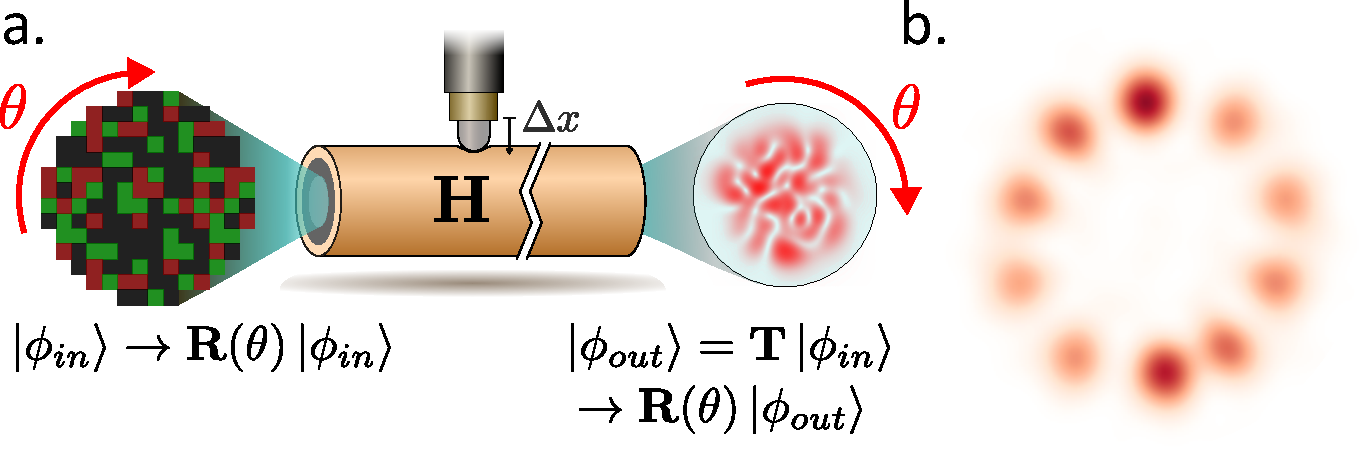
\includegraphics[width=0.99\columnwidth]{images/Fig1.pdf}
\caption{
    \textbf{The rotational memory effect in MMFs.}
    \textbf{a}, Principle of the experiment.
    When the fiber is illuminated by a coherent wavefront $\ket{\phi_{in}}$,
    a seemingly random transmitted field ${\mathbf{T}}\ket{\phi_{in}}$
    is observed at the output.
    In an ideal MMF, due to symmetry, rotating the input wavefront (i.e., sending ${\mathbf{R}(\theta)}\ket{\phi_{in}}$)
    and measuring the transmitted field ${\mathbf{T}\mathbf{R}(\theta)}\ket{\phi_{in}}$,
    is equivalent to rotating the output field for the initial excitation
    ${\mathbf{R}(\theta)\mathbf{T}}\ket{\phi_{in}}$.
    A local perturbation is later added to study its effect on the RME.
    \textbf{b}, Rotation of a focal spot.
    To illustrate this effect,
    we focus light at a given output position
    and rotate the input phase mask along the axis of the fiber
    for 10 different rotation angles.
    We sum all the resulting output amplitude patterns.
    We observe the conservation of the focal spot
    with variations in focal intensity
    that are maximal for angles of $0$ and $\pi$.
    % \textbf{The rotational memory effect in MMFs.}
    % \textbf{a}, Principle of the experiment. 
    % When the fiber is illuminated by a coherent wavefront $\ket{\phi_{in}}$, 
    % a seemingly random transmitted field ${\mathbf{T}}\ket{\phi_{in}}$ 
    % is observed at the output.
    % In an ideal MMF, due to symmetry, rotating the input wavefront, 
    % i.e. sending ${\mathbf{R}(\theta)}\ket{\phi_{in}}$, 
    % and measuring the transmitted field ${\mathbf{T}\mathbf{R}(\theta)}\ket{\phi_{in}}$, 
    %  is equivalent to rotating the output field for the initial excitation
    %  ${\mathbf{R}(\theta)\mathbf{T}}\ket{\phi_{in}}$. 
    %  A local perturbation is later added to study its effect on the RME.
    % \textbf{b}, Rotation of a focal spot.
    % To illustrate this effect, 
    % we focus light at a given output position, 
    % and rotate the input phase mask along the axis of the fiber 
    % for 10 different rotation angles.
    % We sum all the resulting output amplitude patterns. 
    % We observe conservation of the focal spot 
    % with variations of the focal intensity 
    % that is maximal for $0$ and $\pi$.
}
\label{fig:setupSimple}
\end{figure}


 
%  We characterize this effect by sending a set of random patterns
%  on the input facet of the fiber, 
%  rotating this wavefront, and measuring the complex field. 
%  To study the effect of perturbations, 
%  we introduce a local deformation $\Delta x$. 
%  \textbf{b}, Experimental measure of the correlation $C(\theta)$ between 
%  ${\mathbf{T}\mathbf{R}(\theta)}\ket{\phi_{in}}$
%  and 
%  ${\mathbf{R}(\theta)\mathbf{T}}\ket{\phi_{in}}$
%  for different values of the deformation $\Delta x$. 
%  Results are averaged over $X$ random input illuminations.
% WRONG. TO UPDATE}


\subsection{Measure of the RME}

% To illustrate the effect of the RME, 
% we first observe its effect on a focusing operation.
% We compute from the TM the mask that focuses light at a given position 
% in the output facet of the fiber~\cite{Popoff2010Measuring,Cizmar2011shaping}.
% We note that for this step the knowledge of the TM is not necessary 
% as focusing can be achieved using a sequential optimization~\cite{vellekoop2007focusing,Cizmar2010insitu}
% or phase conjugation~\cite{papadopoulos2012focusing}.
To illustrate the effect of the RME, 
we first observe its impact on a focusing operation. 
We compute the mask that focuses light at a specific position in the output facet of the fiber 
using the TM~\cite{Popoff2010Measuring,Cizmar2011shaping}. 
It is noteworthy that for this step, the knowledge of the TM is not necessary, 
as focusing can be achieved through methods
like sequential optimization~\cite{vellekoop2007focusing,Cizmar2010insitu} 
or phase conjugation~\cite{papadopoulos2012focusing}.
% Then, knowing the transformation between the modulator plane 
% and the input facet of the fiber~\cite{matthes2021learning}, 
% we compute the masks that rotate the input field in this plane 
% (see Appendix X for details). 
%%%
We then rotate the input wavefront.
We show in Fig.~\ref{fig:setupSimple}.b. the sum of the resulting output amplitude patterns 
for 10 values of the rotation angle. 
We see that rotating the input masks allows rotating the focusing spot 
along the optical axis of the fiber with limited degradation of the focusing quality.\\
% We then rotate the input wavefront.
% We show in Fig.~\ref{fig:setupSimple}.b. the sum of the resulting output intensity patterns 
% for 10 values of the rotation angle. 
% We see that rotating the input masks allows rotating the focusing spot 
% along the optical axis of the fiber with small degradation of the focusing quality.\\

% To further characterize the RME, 
% we want to quantify the similarity, 
% for an input field $\ket{\phi}$, 
% between a  transmitted field pattern with a rotation of the input field 
% by an angle $\theta$,
% $\mathbf{T}\mathbf{R(\theta)}\ket{\phi}$,
% and the transmitted field rotated by the same angle,  
% $\mathbf{R(\theta)}\mathbf{T}\ket{\phi}$.
To further characterize the RME, we seek to quantify the similarity 
between a transmitted field $\mathbf{T}\ket{\phi}$
for a normalized input field $\ket{\phi}$, 
and the output field $\mathbf{t}(\theta)\ket{\phi}$
for the same input, but rotated by an angle $\theta$
and subsequently rotated back by an angle $-\theta$ at the output.
We define a correlation coefficient for this purpose as follows~\cite{yilmaz2021customizing}:

\begin{equation}
    C(\theta) = 
    \left|
    \frac{
        \bra{\phi}\mathbf{T}^\dagger\mathbf{t}(\theta)\ket{\phi}
    }{
        \sqrt{
            % \bra{\phi}\mathbf{T}^\dagger\mathbf{T}\ket{\phi}
            % \bra{\phi}\mathbf{R(\theta)}^\dagger\mathbf{T}^\dagger\mathbf{T}\mathbf{R(\theta)}\ket{\phi}
            \bra{\phi}\mathbf{t}^\dagger(\theta)\mathbf{t}(\theta)\ket{\phi}
        }   
    }
    \right| \, ,
    \label{eq:corr_function}
\end{equation}

\noindent with $\mathbf{t}(\theta) = \mathbf{R(-\theta)}\mathbf{T}\mathbf{R(\theta)}$.

% In practice, we send a set of $100$ random input wavefronts, 
% rotate them in the plane of the input facet,
% measure the output field,
% and compute the average the correlation coefficient $\left\langle C(\theta)\right\rangle$. 
% We show in Fig.~\ref{fig:correlation}(a, {color} curve) experimentally measured $\left\langle C(\theta)\right\rangle$ 
% for the fiber without added perturbation. 
% We emphasize that for characterizing the memory effect, the measure of the TM is not used, 
% only the knowledge of the input aberration and misalignment effects is exploited 
% to accurately rotate the input field.
In practice, we send a set of $100$ random input wavefronts, 
rotate them in the plane of the input facet,
and measure the output field.
We then compute the average correlation coefficient $\left\langle C(\theta)\right\rangle$. 
Figure~\ref{fig:correlation} (bright red curve) 
shows the experimentally measured $\left\langle C(\theta)\right\rangle$ 
for the unperturbed fiber.
% along with the measurements for the same fiber with gradually applied deformation (red to brown).
We emphasize that the measurement of the TM is not utilized for characterizing the memory effect; 
only the knowledge of the input aberration and misalignment effects is exploited 
to accurately rotate the input field.
While the results shown here correspond to complex field correlations, 
we demonstrate in Appendix B that similar results are obtained 
for intensity correlation measurements. 
This observation is consistent with what was originally presented in~\cite{amitonova2015rotational},
where the intensity RME correlation can be expressed as $C_I(\theta) \approx C(\theta)^2$. 
Furthermore, we show in Appendix B that when the TM is known, 
the RME correlation can be accurately computed without the need for additional measurements.
% While the results shown here correspond to complex field correlations, 
% we show in Appendix B that similar results are obtained 
% for intensity correlation measurements, 
% as originally presented in~\cite{amitonova2015rotational},
% using the fact that the 
% intensity RME correlation can be expressed $C_I(\theta) \approx C(\theta)^2$. 
% Moreover, we also show in Appendix B that when the TM is known, 
% the RME correlation can be computed without additional measurements. 

\begin{figure}[ht]
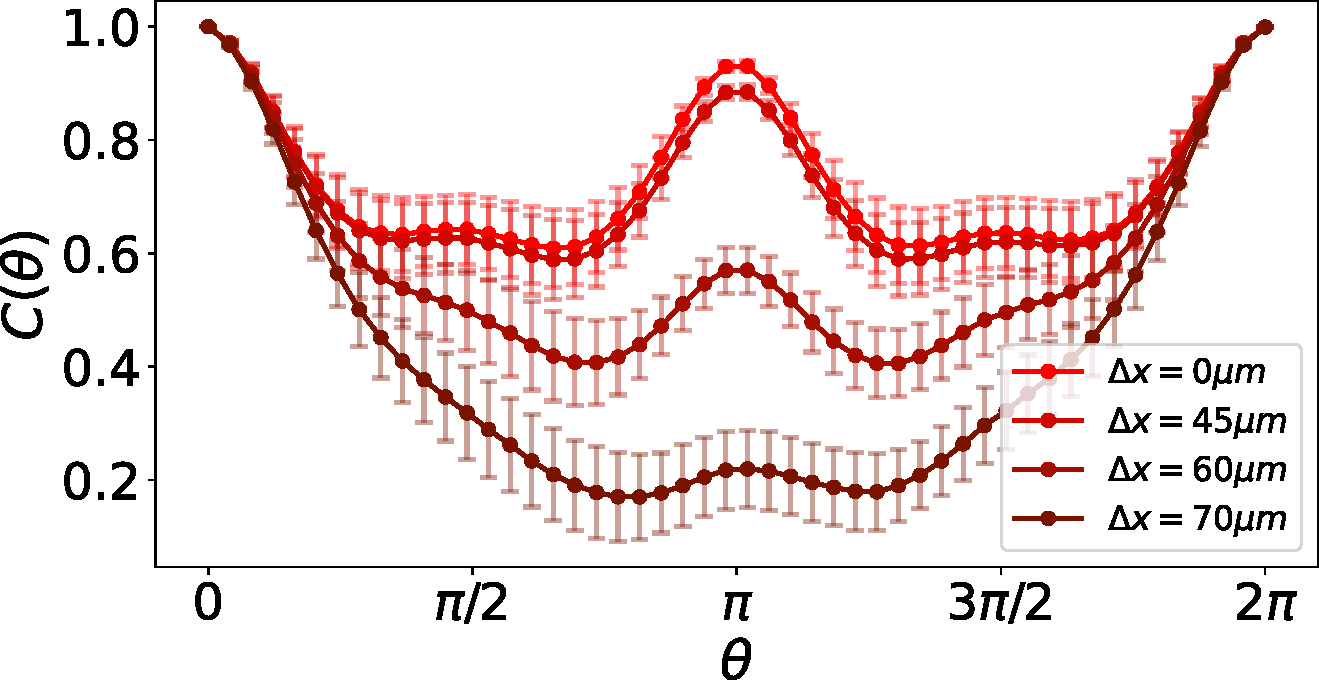
\includegraphics[width=0.49\textwidth]{images/Fig2.pdf}
\caption{
\textbf{Experimental measure of the RME angular correlation as a function of the level of perturbation.}
    Correlation between the rotated output pattern and the output for a rotated input pattern of the same angle $\theta$, 
    as defined in Eq.~\ref{eq:corr_function}. 
    The bright red curve shows results for the unperturbed fiber.
    Red to brown curves correspond to gradually added perturbations 
    by applying a local deformation with a translation stage.
}
\label{fig:correlation}
\end{figure}

% To study the effect of perturbations on the RME, 
% we gradually apply a controlled deformation on the fiber 
% along an axis orthogonal to the propagation direction. 
% The correlation curves as a function of the rotation angle $\theta$ 
% are presented in Fig.~\ref{fig:setupSimple}(b). 

To study the effect of perturbations on the RME, 
we gradually apply a controlled deformation to the fiber 
along an axis orthogonal to the propagation direction. 
\blue{
    The fiber is maintained on a V-groove and we press locally on the fiber from the top
    with a spherical metallic tip using a motorized translation stage.
}
The correlation curves, as a function of the rotation angle $\theta$, 
are presented in Fig.~\ref{fig:correlation} (red to brown curves). 


\subsection{Observations}

% We first observe that, even without applying a perturbation of the fiber, 
% the correlation decreases down to $\sim 60\%$ 
% for values of $\theta$ close to $\pm\pi/2$.
% As the fiber is held straight, 
% this can be attributed to the presence defects of in the fiber 
% or measurement inaccuracies. 
% The effect of the latter is minimal as we compensate for the aberration and misalignments effects 
% (as detailed in Appendix A.). 
% The agreement with the proposed model in the following confirms this assertion.
% This correlation curve presents a second maximum, close to $95\%$, at $\theta=\pi$ 
% and small local minima at $\theta\pm\pi/2$. 
% These features are signatures of the geometrical defects of the fiber.
% When the deformation is applied, 
% we observe the correlation as a function of $\theta$ globally decreases  
% and that the local minima disappear. 

We first observe that, even without applying a perturbation to the fiber, 
the correlation decreases to approximately $60\%$. 
% for values of $\theta$ close to $\pm\pi/2$.
When the fiber is held straight, 
this effect can be attributed to the presence of defects in the fiber. 
% or to measurement inaccuracies. 
% The impact of the latter is minimal, as we compensate for aberrations and misalignments 
% (as detailed in Appendix A). 
% The subsequent agreement with our proposed model confirms this observation.
This correlation curve exhibits a second maximum, close to $95\%$, at $\theta=\pi$, 
along with small local maxima at $\theta\pm\pi/2$ and $3\theta\pm\pi/2$. 
These features are indicative of the geometrical defects within the fiber.
Upon applying the deformation, 
we observe that the correlation as a function of $\theta$ decreases globally, 
and the local maxima vanish. 

% To further understand these effects, 
% we develop a simple model to predict and explain 
% the behavior of the RME in the presence of small perturbations 
% and compare its predictions to the observations.
To further understand these effects, 
we develop a theoretical model to predict and elucidate 
the behavior of the RME in the presence of minor perturbations, 
comparing its predictions to our experimental observations.

% The first effect, we call the \textit{revival effect}, does not deteriorate the correlation at $\theta = \pi$, 
% and seems to have a constant width.

\section{II. Effect of disorder on the RME}

 \subsection*{Model}

% In an ideal MMF, 
% due to the axisymmetry of the system, 
% one should observe a perfect RME, 
% i.e. rotating a given input wavefront 
% has the effect of rotating the output wavefront. 
% \red{However, real fibers are not perfect, 
% leading to mode coupling 
% that is dominated by the effect of 
% geometrical defects of the fibers~\cite{ho2013mode}. 
% We can identify two main contributions: 
% large radius bends, 
% due to the geometrical conformation of the fiber
% and small distortions of the core-cladding interface, 
% mainly due to fabrication inaccuracies~\cite{Marcuse1973coupled}.
% [add input from Lille]}\\

% Let's now consider perturbations characterized by a potential 
% representing the deviation of the index profile from a perfect axisymmetric function 
% of the form 

In an ideal MMF, 
due to the axisymmetry of the system, 
one should expect a perfect RME, 
\blue{
i.e. when
} rotating a given input wavefront 
results in a corresponding rotation of the output wavefront. 
However, real fibers are seldom perfect, 
leading to mode coupling 
that is principally influenced by the 
geometrical defects of the fibers~\cite{ho2013mode}. 
Two main contributions can be identified: 
large radius bends, 
attributable to the geometrical conformation of the fiber,
and minor distortions at the core-cladding interface, 
primarily stemming from fabrication inaccuracies~\cite{Marcuse1973coupled, Mazumder2004analysis, bsaibes2023coupling}.

Let us now consider perturbations characterized by a potential 
that represents the deviation of the index profile from a perfect axisymmetric function 
of the following form:


\begin{equation}
    \delta n(r,\phi, z) = f(z)g(r) \sum_q \Gamma_q\cos(q\phi) \, ,
    \label{eq:disorder}
\end{equation} 
with $q$ integer values and 
$z$, $r$, and $\phi$ the cylindrical coordinates 
corresponding respectively to the longitudinal direction (axis of the fiber), 
the radial, and the azimuthal coordinates. 

% More general deformations can be obtained by decomposing the azimuthal dependence  
% in series of terms $\cos(p\phi)$/$\sin(q\phi)$.
%%
% The longitudinal variation $f(z)$ is characterized by random fluctuations with 
% a correlation length $l_z$, 
% \red{which is typically of the order of $\approx 200$\textmu m [citation from Lille?].} 

% \red{A known effect of the limited accuracy of standard fabrication techniques
% is the difficulty to obtain a precise desired radial index profile, 
% especially for sharp index changes and when close to the core center~[CITATION].
% } 
% \so{This average radial index variation changes the shape of the modes 
% but does not, as the axisymmetry is conserved, affect the RME. 
% It corresponds to an azimuthal deformation function $h(\theta)$
% with $p=0$.
% We will then neglect this effect in this study.}
% % \subsection*{Effect of small fabrication inaccuracies}

% We approximate our fiber of length $L$
% by dividing it into $N_z = \lfloor L/l_z \rfloor$ 
% segments of length $l_z$
% in which the perturbation term $\delta n$ is invariant in $z$, i.e.
% $\delta n_p(r,\phi) = g_p(r)\sum_q \Gamma_q\cos(q\phi)$ for 
% $z \in \left[ p\,l_z, (p+1)l_z \right]$.

% We assume that the radial fluctuations originate from variations between neighboring radial layers caused by inaccuracies in the \textcolor{red}{XXX deposition technique, [citations?]}. 
% We thus model $g_p(r)$
% as a random variable with a 
% correlation $d_\text{layer}$ and a
% standard deviation of $g_p(r)$ as $\sigma_g(r) = d_\text{layer}\frac{dn_0(r)}{dr}$, where $n_0(r)$ represents the radial profile of the unperturbed fiber, and $d_\text{layer}\approx 1$\textmu m corresponds to the thickness of the deposited layers.\\

The longitudinal variation $f(z)$ is characterized by random fluctuations with 
a correlation length $l_z$, 
which is typically on the order of $\approx 100$~\textmu m \red{[citation from Lille?]}.

\blue{
Different fabrication techniques are employed 
based on the fiber type and manufacturer. 
These methods include 
Modified Chemical Vapor Deposition (MCVD), 
Vapor Axial Deposition (VAD), Outside Vapor Deposition (OVD), 
and Plasma Chemical Vapor Deposition (PCVD). 
One well-recognized challenge across these techniques, 
attributed to their inherent limitations in precision, 
lies in achieving a highly accurate radial index profile, 
particularly when dealing with sharp index changes.
}
This average radial index variation alters the shape of the modes but does not, assuming the axisymmetry is conserved, affect the RME. 
It corresponds to an azimuthal deformation with $q=0$.
This effect will be neglected in this study.

We approximate the fiber of length $L$ by dividing it into $N_z = \lfloor L/l_z \rfloor$ segments, each of length $l_z$,
where the perturbation term $\delta n$ is invariant in $z$. 
Specifically,
$
\delta n_p(r,\phi) = g_p(r)\sum_q \Gamma_q\cos(q\phi)\ \text{for}\ z \in \left[ p\,l_z, (p+1)l_z \right].
$

\blue{
We attribute the radial fluctuations to variations between neighboring radial layers, 
stemming from inaccuracies in the deposition technique. 
Specifically, in the case of the fiber under investigation, 
these inaccuracies are associated with the Plasma Chemical Vapor Deposition (PCVD) process.
}
Therefore, we model $g_p(r)$ as a random variable characterized by a correlation $d_\text{layer}$ and a standard deviation~\cite{Lydtin1986pcvd} 
$
\sigma_g(r) = d_\text{layer}\frac{dn_0(r)}{dr},
$
where $n_0(r)$ is the radial profile of the unperturbed fiber, and $d_\text{layer} \approx$
\red {TO UPDATE}
~\textmu m~\cite{geittner1989manufacturing}.


% We approximate the fiber of length $L$ by dividing it into $N_z = \lfloor L/l_z \rfloor$ segments of length $l_z$
% in which the perturbation term $\delta n$ is invariant in $z$, i.e.,
% $\delta n_p(r,\phi) = g_p(r)\sum_q \Gamma_q\cos(q\phi)$ for 
% $z \in \left[ p\,l_z, (p+1)l_z \right]$.

% We assume that the radial fluctuations originate from variations between neighboring radial layers of thickness $d_\text{layer}$ 
% caused by inaccuracies in the \textcolor{red}{XXX deposition technique [citations?]}. 
% We thus model $g_p(r)$
% as a random variable with a 
% correlation $d_\text{layer}$ and a
% standard deviation $\sigma_g(r) = d_\text{layer}\frac{dn_0(r)}{dr}$, where $n_0(r)$ represents the radial profile of the unperturbed fiber, and $d_\text{layer}\approx 1$~\textmu m \red{[citation?]}.% corresponds to the thickness of the deposited layers.


% \begin{equation}
%      f(z) = f_p \quad \text{for} \quad z \in \left[ p\,l_z, (p+1)l_z \right] \, .
%      \label{eq:lz}
% \end{equation}
% We show in Appendix~C
% ~\cite{supp} 
The TM of the $p^\text{th}$ segment of length $l_z$
expressed in the unperturbed fiber mode basis
can be written:

\begin{equation}
    % \mathbf{T} \approx e^{i\left[\mathbf{H}_0 + \mathbf{H}_b\right]L} \, , 
    \mathbf{t}_p = e^{i \left(
                            \mathbf{H}_0 + \mathbf{V}
                        \right) l_z
                     } 
    \, .
    \label{eq:hamiltonian}
\end{equation}



 
%  $\mathbf{H}_0$ is the propagation operator in the absence of perturbation.
% It is a diagonal matrix containing the propagation constants $\beta_\mu$ 
% of the modes of the unperturbed fiber indexed by $\mu$.
% $\mathbf{V}$ represents the perturbation 
% $\frac{2\pi}{\lambda}\delta n_p(r,\phi)$ 
% projected on the mode basis. 
% The full TM is obtained by taking 
% the product of the TMs of all the segments.
$\mathbf{H}_0$ is the propagation operator in the absence of perturbation. 
It is a diagonal matrix containing the propagation constants $\beta_\mu$ 
of the modes of the unperturbed fiber, indexed by $\mu$. 
$\mathbf{V}$ represents the perturbation term 
$
\frac{2\pi}{\lambda}\delta n_p(r,\phi),
$
projected on the mode basis. The full transmission matrix (TM) is obtained by taking the product of the TMs for all the segments.


 \subsection*{Predictions}

% Using coupled mode theory, we can compute the coupling coefficient 
% between two modes $\mu$ and $\nu$ due to this effect~\cite{Marcuse1973coupled, marcuse2013theory}.
As detailed in Appendix~C, we obtain an expression of the correlator $C(\theta)$:
\begin{equation}
    % \mathbf{T} \approx e^{i\left[\mathbf{H}_0 + \mathbf{H}_b\right]L} \, , 
   C(\theta) = \frac{\tilde{C}(\theta) }{\tilde{C}(0) } \, ,
    \label{eq:theo}
\end{equation}

with

\begin{equation}
    % \mathbf{T} \approx e^{i\left[\mathbf{H}_0 + \mathbf{H}_b\right]L} \, , 
   \tilde{C}(\theta) =
            1+ 
            A\sum_{q,\nu,\mu} \Gamma_q^2 
             \cos(q\theta) 
             % \sum_{\nu,\mu}
             B_{\nu\mu}(q)\, ,
    \label{eq:theo2}
\end{equation}


and

\begin{equation}
    A = (k_0 l_z)^2  d_\text{layer}^3 \frac{L/l_z}{4N_\text{modes}} \, . %\frac{L}{l_z}
\label{eq:A}
\end{equation}

% \begin{equation}
%     % \mathbf{T} \approx e^{i\left[\mathbf{H}_0 + \mathbf{H}_b\right]L} \, , 
%    C(\theta) =
%             1+ (k_0 l_z)^2 \frac{L}{l_z} d_\text{layer}^2 
%             A\sum_{q,\nu,\mu} P(\Gamma_q^2) 
%              \left(\cos(q\theta) -1 \right)
%              % \sum_{\nu,\mu}
%              B_{\nu\mu}(q)\, .
%     \label{eq:theo}
% \end{equation}

% $A$ is a coefficient that depends on the geometrical parameters of the fiber.
% $B_{\nu\mu}(q)$ corresponds to the energy coupling  
% between modes $\nu$ and $\mu$
% introduced by a perturbation of azimuthal periodicity $2\pi/q$~\cite{Marcuse1973coupled, marcuse2013theory}, 
% and is expressed:

$A$ is a coefficient that depends on the geometrical parameters of the fiber.
$B_{\nu\mu}(q)$ corresponds to the energy coupling between modes $\nu$ and $\mu$, 
introduced by a perturbation of azimuthal periodicity $2\pi/q$~\cite{Marcuse1973coupled, marcuse2013theory}, 
and is expressed as:

% L_tot / dz * (k0 * dz) ** 2 * 1 / nmodes * 0.25
% $$
% \frac{1}{N_\text{modes}}
% $$
\begin{equation}
   B_{\nu\mu}(q) = 
        \delta_{|m_\mu-m_\nu|,q} 
        \text{sinc}^2\left(\frac{\beta_\mu-\beta_\nu}{2}\right)
        I_{\nu\mu} \, ,
    \label{eq:coupling}
\end{equation}

with 
\begin{equation}
I_{\nu\mu} = 
    \int_0^\infty dr 
        \left|\psi_\mu(r)\right|^2 
        \left|\psi_\nu(r)\right|^2 
        \sigma^2_g(r) r^2 \, .
\end{equation}


% with $\gamma_q$ the coefficient of the series decomposition 
% of the azimuthal function of the disorder $ h(\theta) = \sum_q \gamma_q\cos(q \theta)$.\\

\subsection*{Validation of the Theory}

% To validate the model, 
% we first find the values of the coefficients $\Gamma_q$ that best fit the experimental data 
% using Eq.~\ref{eq:theo}. 
% For this fiber, it is enough to use 4 coefficient for $q \in [1,2,3,4]$
% to make the correlation curves match, 
% as shown in Fig.~\ref{fig:theoryVSexpVSsimu}.
% To validate the theoretical predictions, 
% we then perform simulations using the values of $\Gamma_q$ found 
% using no additional fitting parameter. 
% The simulation consists in dividing the fiber into segments of length $l_z$. 
% We then estimate using a custom fiber solver~\cite{pyMMF} 
% the TM of each segment with an index profile matching the specifications of the fiber 
% to which we add a perturbation of the form given by Eq.~\ref{eq:disorder}. 
% The full TM of the fiber is then obtained by multiplying the TMs of all the segments.
% We compute the RME correlation as a function of the angle and average over 20 realizations of the fiber.
% Results are presented in Fig.~\ref{fig:theoryVSexpVSsimu}.
% Noticeably, we have a reasonable agreement between simulations and theory 
% without any fitting parameter.
To validate the model, 
we first find the values of the coefficients $\Gamma_q$ that best fit the experimental data 
using Eq.~\ref{eq:theo}. 
For this fiber, it is sufficient to use 4 coefficients for $q \in [1,2,3,4]$
to make the correlation curves match, 
as shown in Fig.~\ref{fig:theoryVSexpVSsimu}.
We then perform simulations using the values of $\Gamma_q$ found, 
with no additional fitting parameters. 
The simulation consists of dividing the fiber into segments of length $l_z$. 
We then estimate, using a custom fiber solver~\cite{pyMMF}, 
the TM of each segment with an index profile matching the specifications of the fiber, 
to which we add a perturbation of the form given by Eq.~\ref{eq:disorder}. 
The full TM of the fiber is then obtained by multiplying the TMs of all the segments.
We compute the RME correlation as a function of the angle and average over 20 realizations of the fiber.
Results are presented in Fig.~\ref{fig:theoryVSexpVSsimu}.
Noticeably, there is a reasonable agreement between the simulations and theory 
without the need for any fitting parameters.


\begin{figure}[ht]
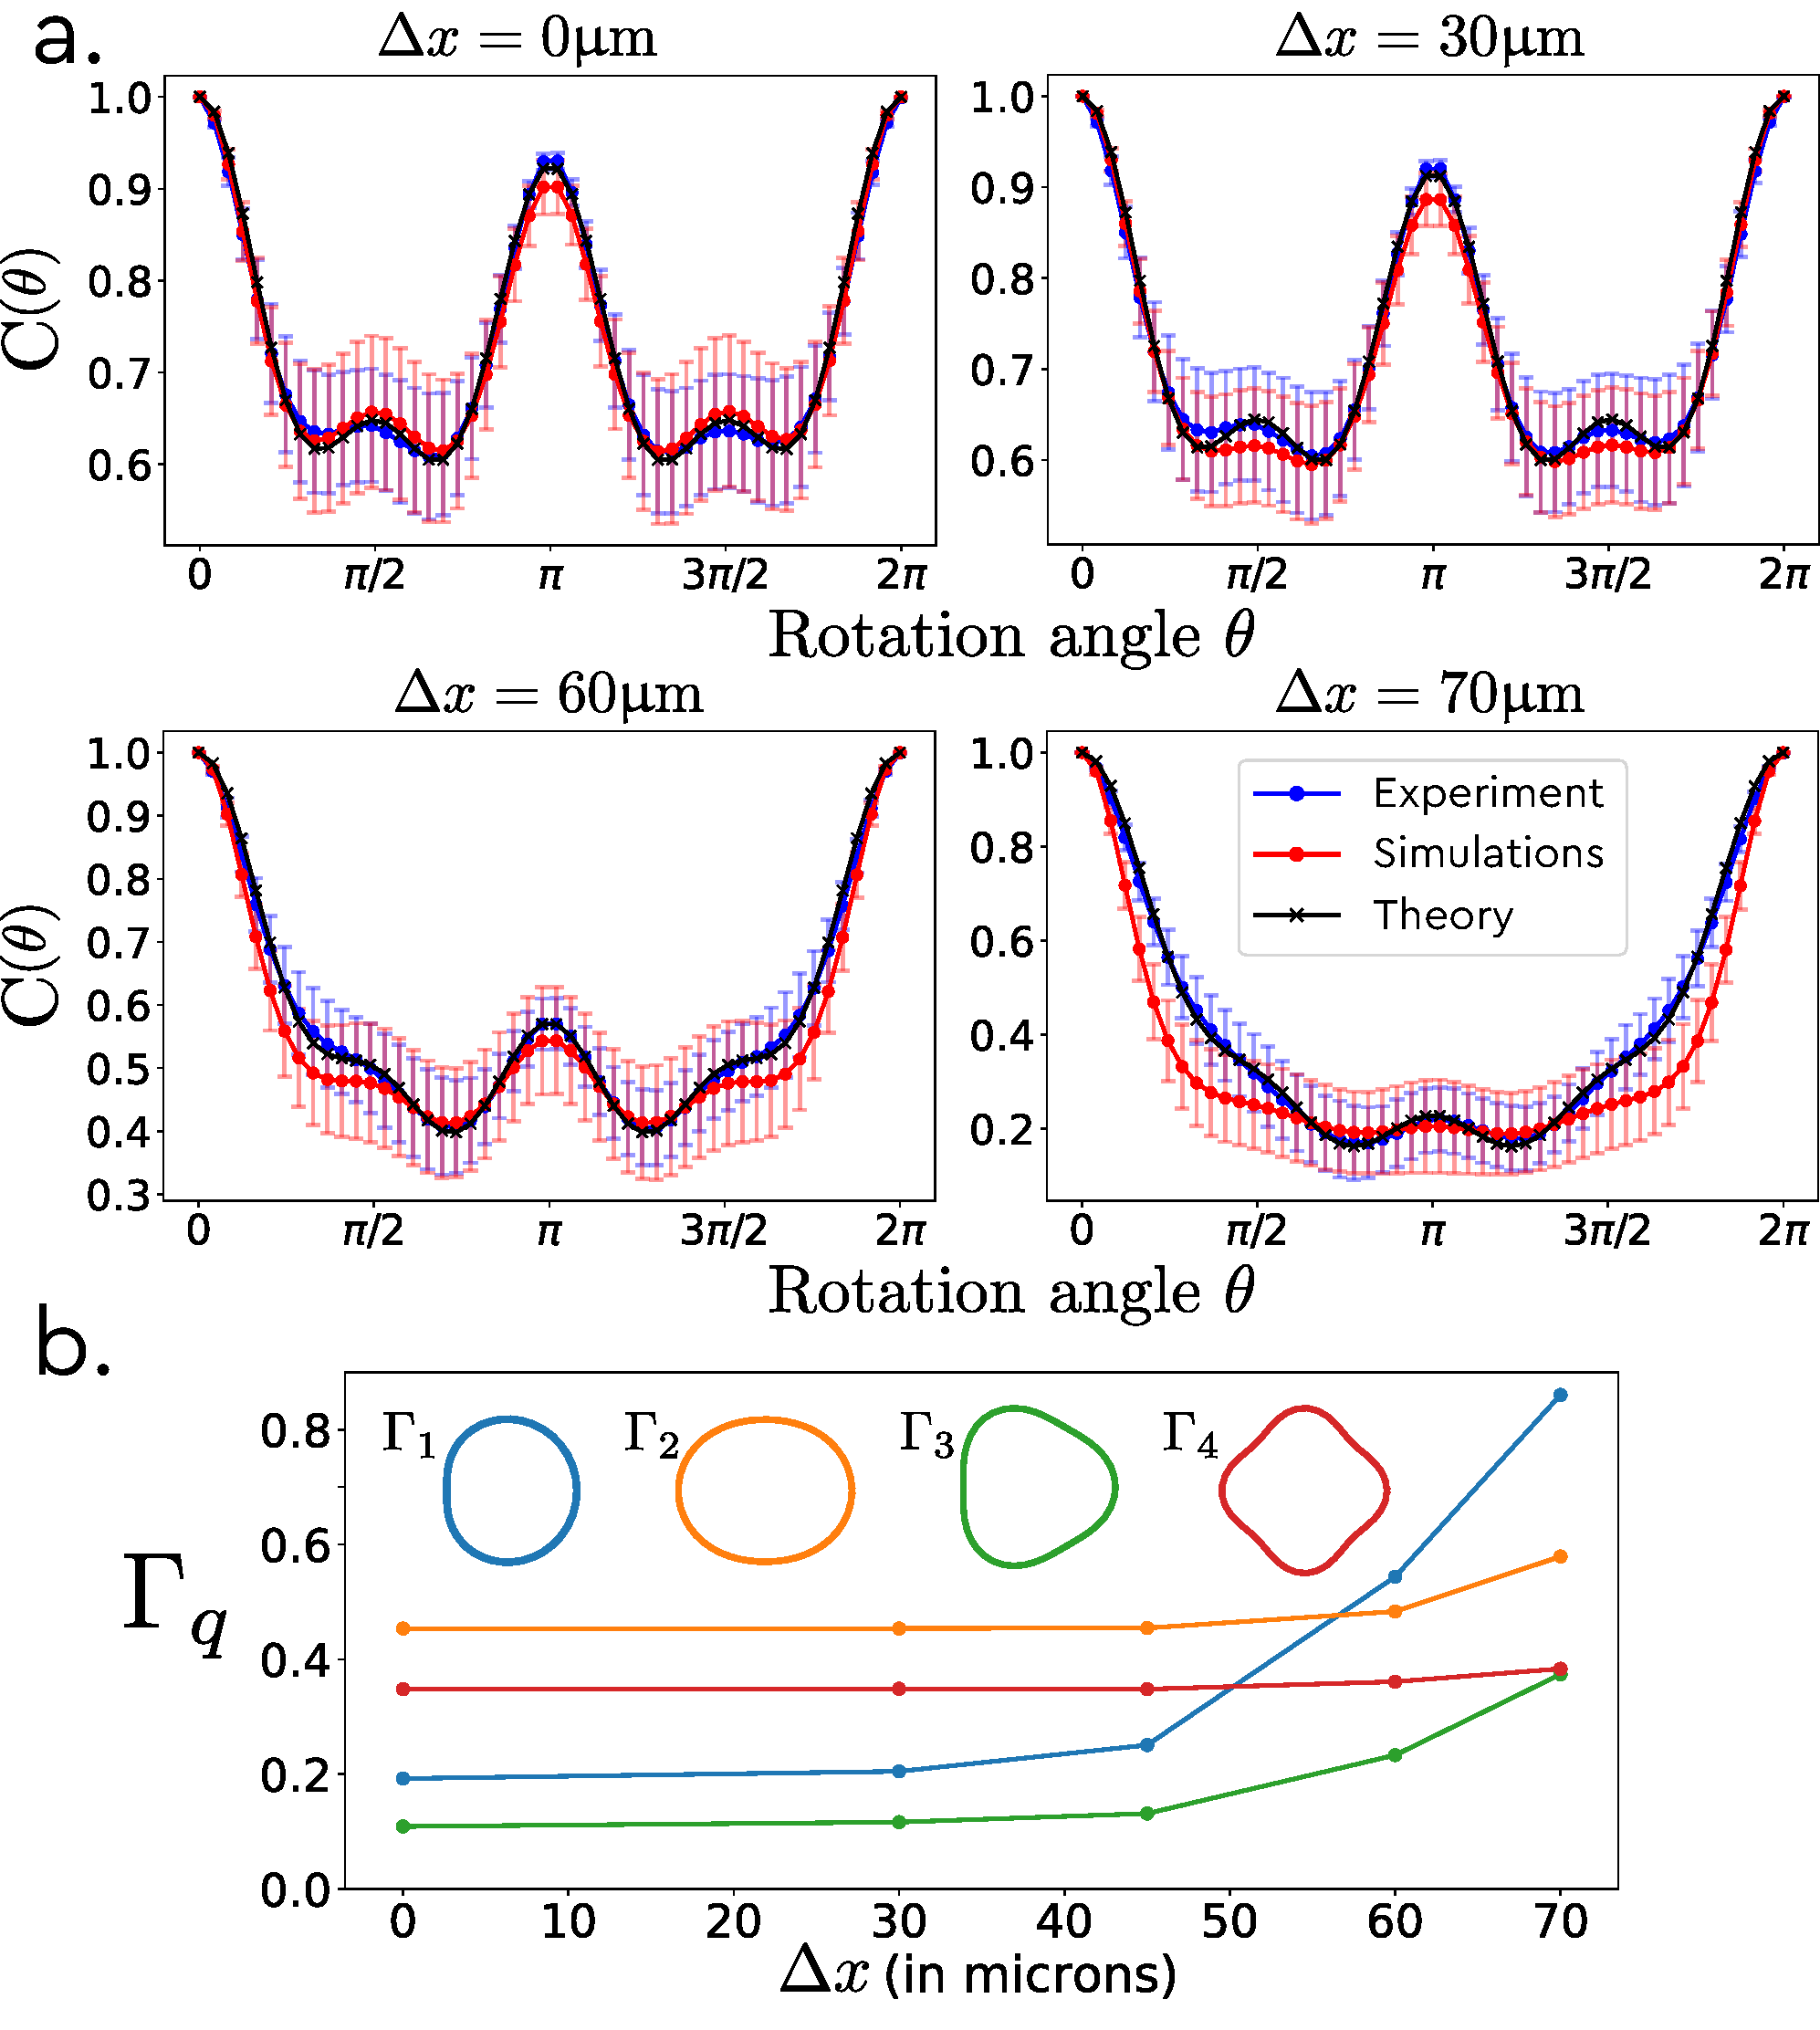
\includegraphics[width=0.49\textwidth]{images/Fig3.pdf}
\caption{
    \textbf{Comparison between experiment, simulations, and theory.}
    a, Correlation curves of the RME, as defined in Eq.~\ref{eq:corr_function},
    for various levels of deformation:
    experimental data (blue),
    fit of the model using Eq.~\ref{eq:theo} (black),
    and simulation results using the same parameters as those for the theoretical model fit (red).
    b, Values of the deformation parameters $\Gamma_q$ found by fitting
    the theoretical model to the experimental data
    as a function of the deformation.
    In the insert, we show the symmetry corresponding to the perturbation associated with each value of $q$.
}
\label{fig:theoryVSexpVSsimu}
\end{figure}

\subsection*{Interpretation}

% The different values of the angular momenta $q$ of the deformation has different 
% origins and impact on the RME. 
% For $\Delta_x = 0$\textmu m, 
% thanks to the prior compensation for aberration effects, 
% the deviation of the correlation curve from a perfect RME 
% ($C(\theta) = 1$)
% is due to the intrinsic defects of the fiber 
% due to the fabrication process. 
% For $\Delta_x > 0$\textmu m,
% the mechanical deformation is responsible for the gradual destruction 
% if the RME, 
% and in particular the disappearing of the revival effect at $\theta = \pi$.\\

The different values of the angular momenta \(q\) of the deformation have different
origins and impacts on the RME.
For \(\Delta_x = 0\)~\textmu m,
thanks to the prior compensation for aberration effects,
the deviation of the correlation curve from a perfect RME
(\(C(\theta) = 1\))
is due to the intrinsic defects of the fiber
caused by the fabrication process.
For \(\Delta_x > 0\)~\textmu m,
the mechanical deformation is responsible for the gradual destruction
of the RME,
and in particular, the disappearance of the revival effect at \(\theta = \pi\).\\



% In the absence of additional perturbation, 
% the correlation curve is dominated by the effect of even values of $q$, 
% which are responsible for the dips at $\theta = \pi \pm \pi/2$ ($q = 2$)
% and the ones at $\theta = \pi/2 \pm \pi/4$ and  $\theta = 3\pi/2 \pm \pi/4$ ($q = 4$). 
% In particular, all even contributions lead to a revival peak at $\theta = \pi$.
% The odd contributions are responsible for the small decay of the correlation at $\theta=\pi$.
% While all the terms are of the same order of magnitude, 
% their effect is much smaller. 
% This is explained by the modal properties of the fiber.
% \red{Indeed, quasi-degenerate groups of modes in graded-index fibers all have the same parity 
% of the orbital angular momentum $m$~[REF].}
% In equation~\ref{eq:theo}, 
% when introducing an odd deformation, 
% we couple modes with different parities of the angular momentum.
% This leads to a significant difference in propagation constants, 
% and then to a small value for the term $\text{sinc}^2\left(\frac{\beta_\mu-\beta_\nu}{2}\right)$, 
% which limits its impact on the RME correlation.
% This explains the robustness of the revival effect observed at $\theta = \pi$.\\

% When the mechanical deformation is introduced, 
% we find that the value of $\Gamma_1$, 
% corresponding to a flattening of the fiber, 
% gradually increases. 
% This explains the disappearance of the revival effect 
% and is consistent with the geometry of the introduced perturbation.

In the absence of additional perturbation,
the correlation curve is dominated by the effect of even values of \(q\),
which are responsible for the dips at \(\theta = \pi \pm \pi/2\) (\(q = 2\))
and the ones at \(\theta = \pi/2 \pm \pi/4\) and \(\theta = 3\pi/2 \pm \pi/4\) (\(q = 4\)).
In particular, all even contributions lead to a revival peak at \(\theta = \pi\).
The odd contributions are responsible for the slight decay of the correlation at \(\theta=\pi\).
Although all the terms are of the same order of magnitude,
their effect is much smaller.
This is explained by the modal properties of the fiber.
Indeed, quasi-degenerate groups of modes in graded-index fibers all have the same parity
of the orbital angular momentum $m$
\blue{
~\cite{Olshansky1975mode}.
}
In equation~\ref{eq:theo},
when introducing an odd deformation,
we couple modes with different parities of the angular momentum.
This leads to a significant difference in propagation constants,
resulting in a small value for the term \(\text{sinc}^2\left(\frac{\beta_\mu-\beta_\nu}{2}\right)\),
which limits its impact on the RME correlation.
\blue{
Coupling between degenerate modes is the dominant effect for small perturbations~\cite{matthes2021learning}.
However, since modes all have the same parity,
it does not break the symmetry by rotation by an angle of $\pi$
(see Appendix D).
}
This explains the robustness of the revival effect observed at \(\theta = \pi\).\\

When the mechanical deformation is introduced,
we find that the value of \(\Gamma_1\),
corresponding to a flattening of the fiber,
gradually increases.
This explains the disappearance of the revival effect
and is consistent with the geometry of the introduced perturbation.\\

\blue{
We show in Appendix F the results for other graded-index fibers 
with similar advertised properties. 
While we obtain comparable results, 
these lead to different contributions of $\Gamma_q$, 
even for different spools of the same fiber. 
This highlights the variations in perturbations 
that occur during the fabrication process, 
but which can be estimated by measuring the RME.
}




%  \subsection*{Agreement with experiment}

% % For two fibers with similar advertised properties ($50$\textmu m-core graded-index with NA$=0.2$), 
% % we use our model to fit the experimental data for the fiber
% % without perturbation by adjusting the values of $\Gamma_q$. 
% % The results are shown in Fig.~\ref{fig:correlation}. 
% % We obtain a good agreement by setting non-zero values for $q=1$ and $2$, 
% % and, for one of the fibers, $q=4$.
% % The $q=1$ contribution is responsible for the small decay of the correlation at $\theta=\pi$.
% % While this term is of the same order of magnitude as the others, 
% % its effect is much smaller. 
% % \red{Indeed, quasi-degenerate groups of modes in graded-index fibers all have the same parity 
% % of the orbital angular momentum $m$~[REF].}
% % In equation~\ref{eq:coupling}, 
% % when introducing a $q=1$ deformation, 
% % we couple modes with an orbital angular momentum difference $\delta m \pm 1$, 
% % which then have different parities of the angular momentum.
% % This leads to a significant difference in propagation constants, 
% % and then to a small value for the term $\text{sinc}^2\left(\frac{\beta_\mu-\beta_\nu}{2}\right)$.

% All even contributions lead to a revival peak at this angle. 
% This can be explained by the symmetry of the modes and the deformation.
% % When introducing a symmetric deformation ($q=1$), we couple modes with an orbital angular momentum difference $\delta m \pm 1$, 
% that leads to coupling to modes between non-degenerate groups of modes, 
% which breaks the symmetry of the RME (see Appendix D. for more details).



% The $q=2$ (resp. $q=4$) contribution is responsible for the local maxima at  $\theta=\pi$ (resp.  $\theta=\pm\pi/2$). 
% When we locally press on the fiber, we then only tune the value of $\gamma_1$ 
% and again retrieve a good agreement with the experimental data.
% This observation is consistent with the symmetry of deformation,  
% and is similar to the bending effect in which the perturbation term 
%  can be expressed  as $\delta n(\vec{r})\propto r \cos(\theta)$~\cite{Ploschner2015seing}. 
%  We show in Fig.~S5 of Appendix C. that the fit value for $\gamma_1$  
%  is proportional to the applied deformation. 

%  \subsection*{Validation of the approach}
 
% This validates the approach and the measurements,
% and supports our claim that it is possible to 
% study the symmetry of the small fabrication inaccuracies 
% by studying the RME in the monochromatic regime. 
% The proportionality between deformation and estimated parameters $\gamma_q$
% further support the possibility of a quantitative study of deformations.




% \section{III. Analysis}

% \subsection{The correlation width of the RME}

% In general, a memory effect is defined with respect to a given transformation of the field is not perfect.
% This means that it has a finite range. 
% It is the case for the angular memory effect in scattering media and multi-core fibers, 
% where the output speckle pattern can be shifted without deformation 
% up to a maximum angle that characterizes its range. 
% It corresponds to $\mathbf{T}$ being a band diagonal matrix 
% when expressed in the eigenspace of the transformation operator, 
% i.e. in the representation of the variable conjugated to the transformation parameter.
% For the angular memory effect, the TM is a random band diagonal matrix in the position $x$ 
% and the range is limited by a maximum angle $\theta_x$.
% The range of the memory effect is inversely proportional to the width of the band~\cite{yilmaz2019angular}.


% In the case of the RME in MMFs, 
% the rotation angle is the conjugate quantity to the orbital angular momentum $m$~\cite{Horodynski2020Optimal}. 
% To study the evolution width of the RME, 
% we only take the contribution from the symmetric deformation, that kills the memory effect at $\theta=\pi$.
% We obtain curves that decrease monotonously with the rotation angle 
% on the interval $\left[0, \pi\right]$. 
% We estimate the angular width of the RME by fitting with Gaussian functions 
% and observe that it decreases when the strength of the perturbation increases. 
% This result is fundamentally different from the behavior of the angular memory effect in scattering media, 
% where the range is only determined by the length of the system for a monochromatic excitation, 
% and is not affected by the strength of the disorder~\cite{}. 

% For small symmetric deformations, we saw that we only have coupling
% between pairs of modes with neighboring angular momentum, 
% i.e. for $\delta m = 1$. 
% When the deformation increases, we start coupling to modes further away in the momentum space, 
% leading to a band diagonal TM with a width that increases with the strength of the deformation.




% % As such, the width of the enlargement of the TM in the $m$ coordinate should be inversely proportional 
% % to the angular range $\delta\theta_\text{RME}$ of the RME~\cite{yilmaz2019angular}.
% % This is due to the fact that there is Fourier transform relation between this two quantities.

% % is symmetric with respect to $\theta = \pi/2$.



% \begin{figure*}[ht]
% 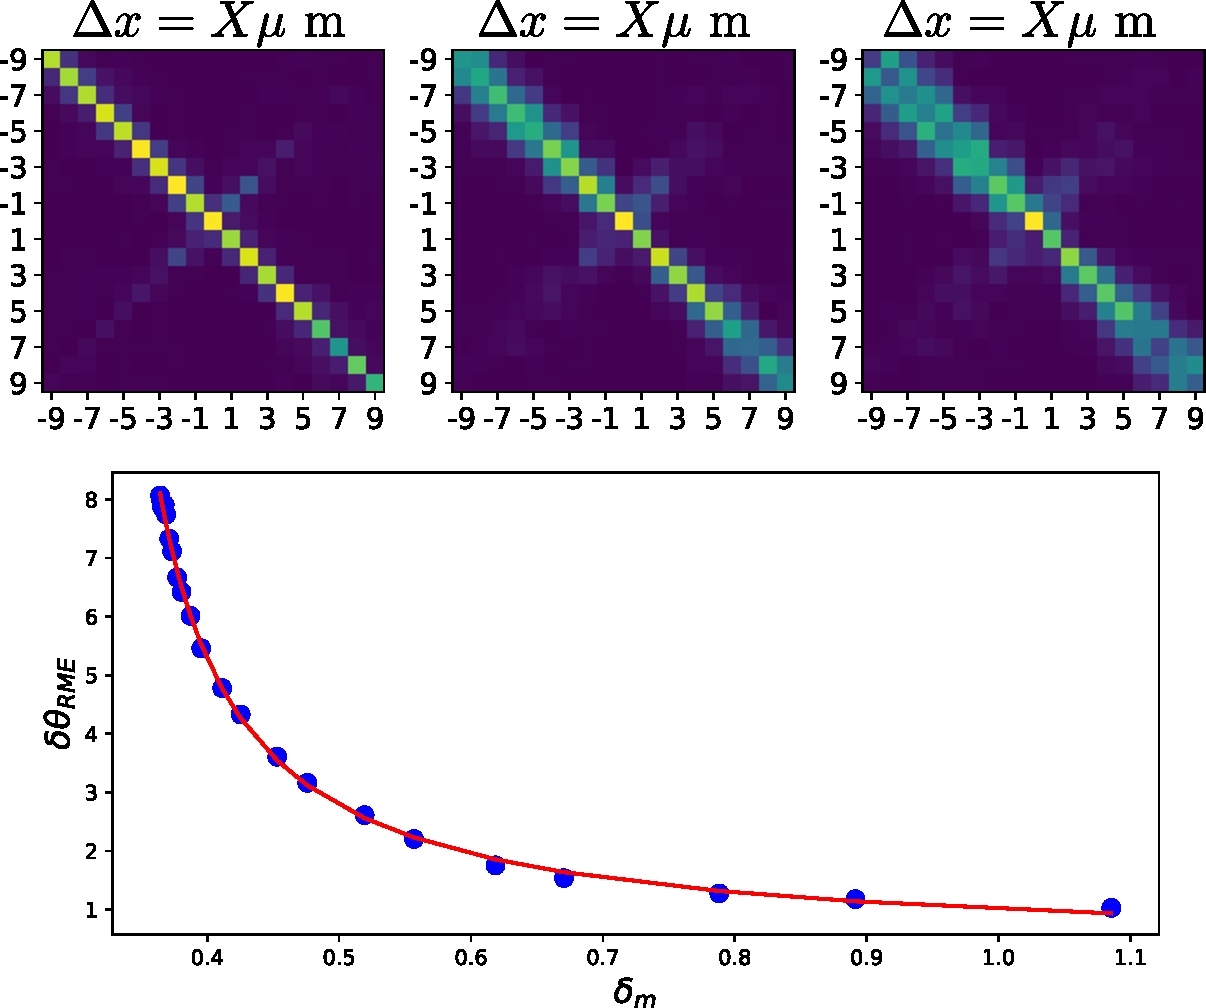
\includegraphics[width=0.95\textwidth]{images/FigDeltaM.pdf}
% \caption{
% \textbf{Width of the diagonal of the transmission matrix in the $m$ space}
% \textbf{a}, a simplified schematic of the experimental setup. 
% }
% \label{fig:width}
% \end{figure*}

% To understand this dependence, we study the mode coupling introduced by a perturbation in the mode basis TM. 
% We show in Fig.~\ref{fig:width}a-c the TM for different values of the deformation. 
% To better illustrate our purpose, we only represent the mode having an radial momentum $l$ equal to 1. 
% The full matrices are represented in Appendix X. 
% We see a broadening of the TM in the angular orbital momentum ($m$) space.
% To quantify it we compute the function
% $
%     I(m') = \left\langle \| h_{ij}\|^2 \right\rangle_{|m_i-m_j| = m'},
% $
% and fit it with a Gaussian function to estimate the width $\delta_m$ 
% as its standard deviation. 
% We show the dependence of the range $\delta\theta_\text{RME}$ of the RME 
% as a function of $\delta_m$ in 
% Fig.~\ref{fig:width}d. 
% Experimental data are closely fitted by a function of the form 
% $\delta\theta_\text{RME} = a+b/(\delta_m-c)$ (red curve) 
% with $c \approx 0.5$, $a \approx X$ and $c \approx X$. 
% BLABLA: --> analyse simulations
% % This shows that the width of the RME does behave as the inverse of the 
% % broadening of the TM in the orbital angular momentum space. 
% % While we demonstrate this dependence for a localized perturbation, 
% % we show in simulations (see Appendix X) 
% % that we obtained a similar behaviour for a global deformation, 
% % in this case of a bent fiber.

\section{III. Tailoring the RME}

% We studied and measured so far the mean correlation 
% $\left\langle C(\theta) \right\rangle$, 
% i.e. obtained when averaging over random input wavefronts.
% We now ask ourselves if it is possible to find specific input wavefronts 
% for which the correlation is significantly higher that the average value 
% for one given angle or for a wide range of angles. 
% Similarly to the approaches to customize the angular memory effect in scattering media~\cite{yilmaz2021customizing}, 
% we can build operators to optimize the memory effect at a given angle. 
% An interesting operator is the one that represents the upper part of the correlation function 
% in Eq.~\ref{eq:corr_function}:
We studied and measured so far the mean correlation 
% $\left\langle C(\theta) \right\rangle$, 
i.e. obtained when averaging over random input wavefronts.
We now ask ourselves if it is possible to find specific input wavefronts 
for which the correlation is significantly higher than the average value 
for one given angle or for a wide range of angles. 
Similarly to the approaches to customize the angular memory effect in scattering media~\cite{yilmaz2021customizing}, 
we can build operators to optimize the memory effect at a given angle. 
An interesting operator is the one that represents the upper part of the correlation function 
in Eq.~\ref{eq:corr_function}:


\begin{equation}
    \mathbf{O}(\theta_t) = \mathbf{T}^\dagger\mathbf{R(\theta_t)}^\dagger\mathbf{T}\mathbf{R(\theta_t)}.
\end{equation}

\begin{figure}[ht]
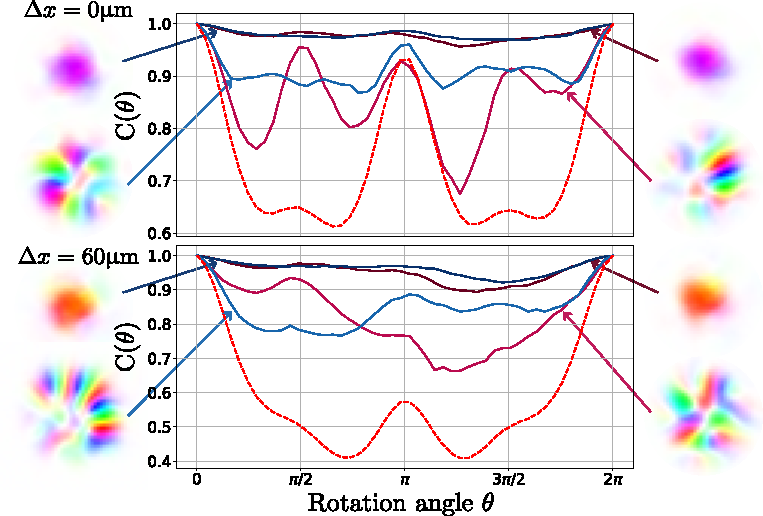
\includegraphics[width=0.49\textwidth]{images/Fig4.pdf}
\caption{
\textbf{Tailoring the rotational memory effect.}
Experimental results for the generation of input channels with 
improved RME range for different values of the deformation.
(add average correlation curve, l'allure des courbes pour l'opérateur commutation est bizarre, ce n'est pas les derniers résultats)
}
\label{fig:tailoring}
\end{figure}

% To optimize the RME correlation for a given target angle $\theta_t$, 
% we first construct this operator using experimentally measured TMs.
% We then compute the eigenvectors of this operator corresponding to the eigenvalue 
% with the largest modulus. 
% We present in Fig.\ref{fig:tailoring} the resulting correlation for 
% the two first eigenvectors of $\mathbf{O}(\theta_t=  \pi/2)$ (shades of pink curves), 
% in the case of no deformation and strong deformations $\Delta x = 60$\textmu m. 
% % We observe a better correlation at the target angle but lower minimal values. 
% The first eigenvector, which stays highly correlated all over the angle range, 
% has a spatial output pattern close to the fundamental mode. 
% The second one presents a local maxima at $\theta = \theta_t$, 
% but also shows oscillation, while always staying over the average correlation curve for random inputs.

% To improve the correlation over the whole $2\pi$ range, 
% we can now study the operator built using the sum of operators describing the correlation at different angles: 

To optimize the RME correlation for a given target angle $\theta_t$, 
we first construct this operator using the experimentally measured TMs.
We then compute the eigenvectors of this operator corresponding to the eigenvalue 
with the largest modulus. 
We present in Fig.~\ref{fig:tailoring} the resulting correlation for 
the two first eigenvectors of $\mathbf{O}(\theta_t = \pi/2)$ (shades of pink curves), 
in the case of no deformation and strong deformations ($\Delta x = 60$~\textmu m). 
% We observe a better correlation at the target angle but lower minimal values. 
The first eigenvector, which remains highly correlated across the entire angle range, 
has a spatial output pattern close to the fundamental mode. 
The second one presents a local maximum at $\theta = \theta_t$, 
but also shows oscillations, while always staying above the average correlation curve for random inputs.

To improve the correlation over the entire $2\pi$ range, 
we can now study the operator built using the sum of operators describing the correlation at different angles:


\begin{equation}
    \mathbf{O}_\text{sum}=\sum_t\mathbf{T}^\dagger\mathbf{R(\theta_t)}^\dagger\mathbf{T}\mathbf{R(\theta_t)} .%\quad \theta_t = t.\pi/2\, , t \in \left[0, 3 \right].
    \label{eq:RME_sum_op}
\end{equation}

% We choose $\theta_t = t\cdot\pi/2$ with $t\in[0.. 3]$. 
% By choosing again the eigenvectors corresponding to the eigenvalues 
% with the largest modulus, 
% we find wavefronts for which the correlation stays highly correlated all over the $2\pi$ range (see Fig~\ref{fig:tailoring}).

% An interesting application to memory effects is the possibility to recover information from the distal side, 
% where the field for a given input wavefront is a priori unknown. 
% For imaging applications, 
% the requirements are both to have a range of the memory effect large enough to cover the size of the object to image, 
% and to have an output excitation with a sharply peaked autocorrelation function~\cite{bertolotti2012non-invasive}. 
% In multiple scattering media, it is guaranteed by the presence of a strong disorder that randomizes the input field 
% for any given input wavefront. 
% In MMFs, the disorder is mode dependent, as it does not affect all the modes the same way~\cite{Cizmar2011shaping}.
% One trivial solution to maximize the range of the RME using the fundamental mode, 
% which is less affected by external perturbations~\cite{matthes2021learning}.
% However, due to its rotational symmetry, its autocorrelation with respect to the angular rotation is close to one. 
% In other words, rotating the pattern does not change the pattern. 
% Thus, even though it stays correlated at the output of the fiber when rotated, 
% it cannot be used to provide information about the distal end of the fiber. 
% % This point is detailed in Appendix XX.%in~\cite{supp}.
% The first eigenvector of each studied operator are very close to the fundamental modes (see inserts in Fig.~\ref{fig:tailoring}). 
% However, the second ones combines the properties of having  a large range RME  
% and a pattern with a peaked autocorrelation function (see Appendix~F). 
% They are then good candidates to be used to recover information about the distal end of the fiber. 

We choose $\theta_t = t\cdot\pi/2$ with $t\in[0, 3]$. 
By selecting the eigenvectors corresponding to the eigenvalues 
with the largest modulus, 
we find wavefronts for which the correlation remains highly correlated across the entire $2\pi$ range (see Fig.~\ref{fig:tailoring}).

An interesting application of memory effects is the possibility to recover information from the distal side, 
where the field for a given input wavefront is a priori unknown. 
For imaging applications, 
the requirements include having a range of the memory effect broad enough to cover the size of the object to be imaged, 
and having an output excitation with a sharply peaked autocorrelation function~\cite{bertolotti2012non-invasive}. 
In multiple scattering media, 
the later is guaranteed by the presence of strong disorder that randomizes the input field 
for any given input wavefront. 
In MMFs, the disorder is mode-dependent, as it does not affect all modes in the same way~\cite{Cizmar2011shaping}.
A trivial solution to maximize the range of the RME involves using the fundamental mode, 
which is less affected by external perturbations~\cite{matthes2021learning}.
However, due to its rotational symmetry, its autocorrelation with respect to angular rotation is close to one. 
In other words, rotating the pattern does not change it. 
Thus, even though it remains correlated at the fiber's output when rotated, 
it cannot be used to provide information about the distal end of the fiber. 
% This point is detailed in Appendix XX.%in~\cite{supp}.
The first eigenvectors of each studied operator are very close to the fundamental modes (see insets in Fig.~\ref{fig:tailoring}). 
However, the second ones combine the properties of having a large-range RME  
and a pattern with a peaked autocorrelation function (see Appendix~F). 
They are therefore good candidates to be used to recover information about the distal end of the fiber.











%The difficulty to accurately measure and characterize the RME 
%is mainly due to the acute sensitivity to slight misalignments and aberrations effects, 
%when, for instance, a simple phase tilt breaks the symmetry of the system.


% is similar to 
% the difficulty to precisely estimate the TM of a fiber. 
% It is mainly due to the acute sensitivity to slight misalignments and aberrations effects~\cite{matthes2021learning}.



% \subsection{TM with disorder}


\section{IV. Conclusion}

In this paper, we first present an approach based on the TM measurement 
to precisely measure and study the RME in MMFs.
Importantly, this method allows us to mitigate the effects of aberrations and misalignments 
that can drastically perturb its estimation. 
We then introduce a theoretical model that is in good agreement with experimental data 
and simulations. 
Noticeably, this model enables the estimation of geometrical perturbations in the fiber, 
whether due to fabrication imperfections or mechanical deformations. 
This approach can serve as a powerful tool for studying MMF defects 
arising from the breaking of the fiber's symmetry. 
Finally, we demonstrate the possibility of generating channels that show
a drastic improvement in the RME. 
In particular, we can create channels that 
are more robust to deformations compared to random inputs or standard fiber modes, 
and also exhibit a random profile with high spatial frequencies. 
This last feature is essential for utilizing the memory effect for blind image recovery~\cite{bertolotti2012non-invasive}.
It paves the way for its use in endoscopy applications, where the perturbation of the fiber changes over time
and access to the distal end is impossible. 
The utilization of the RME also holds great promise for classical or quantum optical telecommunications, 
as the RME could be employed to encode data through the fiber.


% In this paper, we first present an approach based on the TM measurement 
% to precisely measure and study the RME in MMFs.
% Importantly, it allows mitigate the effect of aberrations and misalignments 
% that can drastically perturb its estimation. 
% We then introduce a theoretical model in good agreement with experimental data 
% and simulations. 
% Noticeably, it allows estimating the geometrical perturbation of the fiber, 
% either due to fabrication imperfections or mechanical deformation. 
% This approach can serve as a powerful tool for studying MMF defects 
% due to the breaking of the symmetry of the fiber. 
% Finally, we show the possibility to generate channels that shows
% a drastic improvement of the RME. 
% In particular, we can generate channels that 
% are more robust to deformation compared to random inputs or fiber modes, 
% but also present a random profile with high spatial frequencies. 
% This last feature is essential for using memory effect for blind image recovery~\cite{bertolotti2012non-invasive}.
% It opens the road of its use for endoscopy applications, where the perturbation of the fiber changes over time
% and for which access to the distal end is impossible. 
% The use of the RME also holds great promises for classical or quantum optical telecommunications, 
% as the RME could be used to encode data through the fiber.



\section*{Data and code availability}

\noindent Raw and processed data, sources to regenerate the all the figures,
and sample codes for the treatment pre- and post-processing are  available in the dedicated repository~\cite{repo}.




%%%%%%%%%%%%%%%%%%%%%%%%%%%%%%%%%%%%%%%%%%%%%%%%%%%%%%%%%%%%%%%%%%%%
%%%%%%%%%%%%%%%%%%%%%%%%%%% ANNEXE A %%%%%%%%%%%%%%%%%%%%%%%%%%%%%%%
%%%%%%%%%%%%%%%%%%%%%%%%%%%%%%%%%%%%%%%%%%%%%%%%%%%%%%%%%%%%%%%%%%%%
\section*{ANNEX A: Experimental measure of the TM}

\subsection{Aberration compensation}

% To decouple the effect of the RME and measurement inaccuracies, we use the approach we developed 
% to learn and compensate for aberrations and misalignments~\cite{matthes2021learning}. 
% The idea is to first measure the TM in a pixel basis and then project it onto the mode basis. 
% Without aberrations, the projection in the mode basis should conserve the energy of the TM, 
% as all the energy has to be conveyed by those modes. 
% Using a model based algorithm built using the deep-learning framework PyTorch~\cite{NIPS2019_9015}, 
% we find the aberrations and misalignments of the system that minimized the loss when projection onto the mode basis.
% It allows us to recover accurately the TM in the mode basis. 
% This object possess all the information about light propagation in the MMF.
To decouple the effects of the RME and measurement inaccuracies, we utilize the approach we developed 
to learn and compensate for aberrations and misalignments~\cite{matthes2021learning}. 
The idea is to first measure the TM on a pixel basis and then project it onto the mode basis. 
Without aberrations, this projection into the mode basis should conserve the energy of the TM, 
since all the energy must be conveyed by those modes. 
Using a model-based algorithm, constructed with the deep-learning framework PyTorch~\cite{NIPS2019_9015}, 
we identify the aberrations and misalignments of the system that minimize the loss when projecting onto the mode basis.
First, this process enables us to accurately recover the TM in the mode basis, 
which contains all the information about light propagation in the MMF. 
Secondly, it facilitates the identification of the aberrations that need to be corrected 
in order to obtain a desired pattern in the input facet plane of the fiber. 
The correction can then be implemented onto the modulator.



% with a typical width that decrease when the perturbation increases.

%%%%%%%%%%%%%%%%%%%%%%%%%%%%%%%%%%%%%%%%%%%%%%%%%%%%%%%%%%%%%%%%%%%%
%%%%%%%%%%%%%%%%%%%%%%%%%%% ANNEXE B %%%%%%%%%%%%%%%%%%%%%%%%%%%%%%%
%%%%%%%%%%%%%%%%%%%%%%%%%%%%%%%%%%%%%%%%%%%%%%%%%%%%%%%%%%%%%%%%%%%%
\section*{Appendix B: Correlation estimation of the RME in different configurations}

\subsection*{Intensity vs field correlation}

We compare the field correlation, as utilized in the rest of this work, 
with the square root of the intensity correlation, 
as demonstrated in the original RME observation~\cite{amitonova2015rotational}. 
As illustrated in Fig.~\ref{fig:CEvsCI}, the two correlations are in excellent agreement, 
demonstrating that these observables are equivalent.




\begin{figure}[ht]
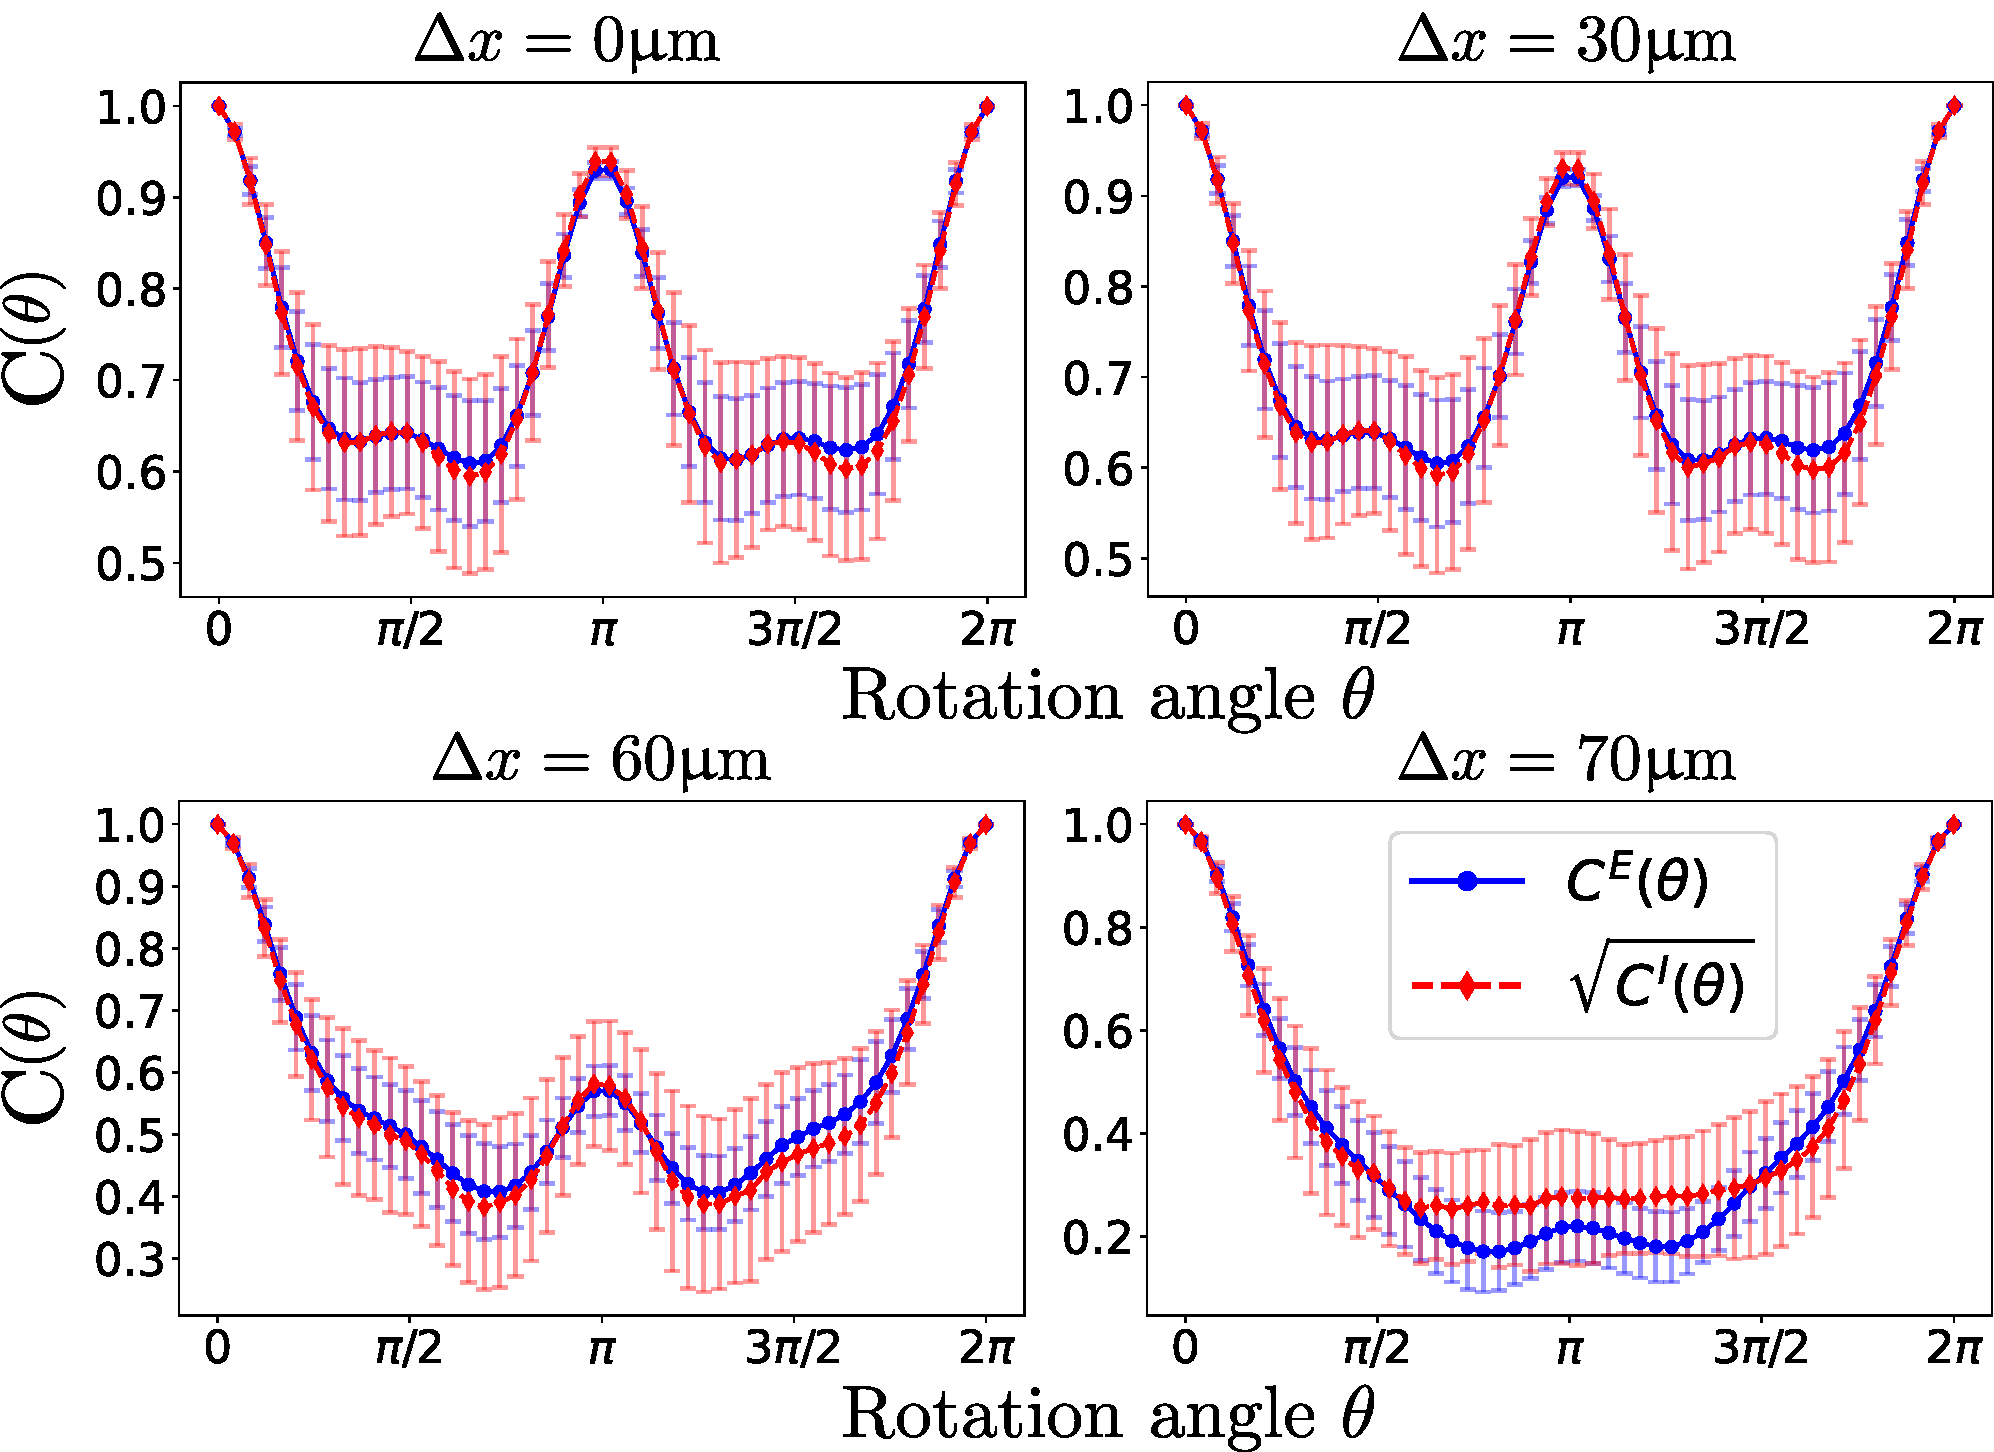
\includegraphics[width=0.49\textwidth]{images/Fig_A1.pdf}
\caption{
    \textbf{Comparison between the intensity and the field correlation as a function of the rotation angle.}
    For different values of the deformation, 
    we show the field correlation as defined in Eq.~\ref{eq:corr_function} (blue curve), 
    and the square root of the intensity correlation with the same data (red curve).
}
\label{fig:CEvsCI}
\end{figure}

\subsection*{Estimation of the correlation using the measured TM}

In the study presented,
we utilize the compensation of aberrations, facilitated by the transmission matrix (TM) measurement,
but we do not directly employ the knowledge of the TM itself.
However, the TM provides access to the output field $\ket{\phi_{\text{out}}}$
for any given input field $\ket{\phi_{\text{in}}}$.
We can then use the TM to estimate the output of a rotated wavefront.
To estimate the RME (Rotated Mode Entanglement) correlation, we numerically simulate the experiment performed.
For each deformation, we compute the correlation between the output field for a rotated wavefront and the output field for the original one, across 100 random input wavefronts.
We show in Fig.~\ref{fig:TMvsCE} a good agreement,
demonstrating that the measurement of the TM can drastically reduce
the time needed for characterizing the RME, 
as it does not require any additional measurement.

\begin{figure}[ht]
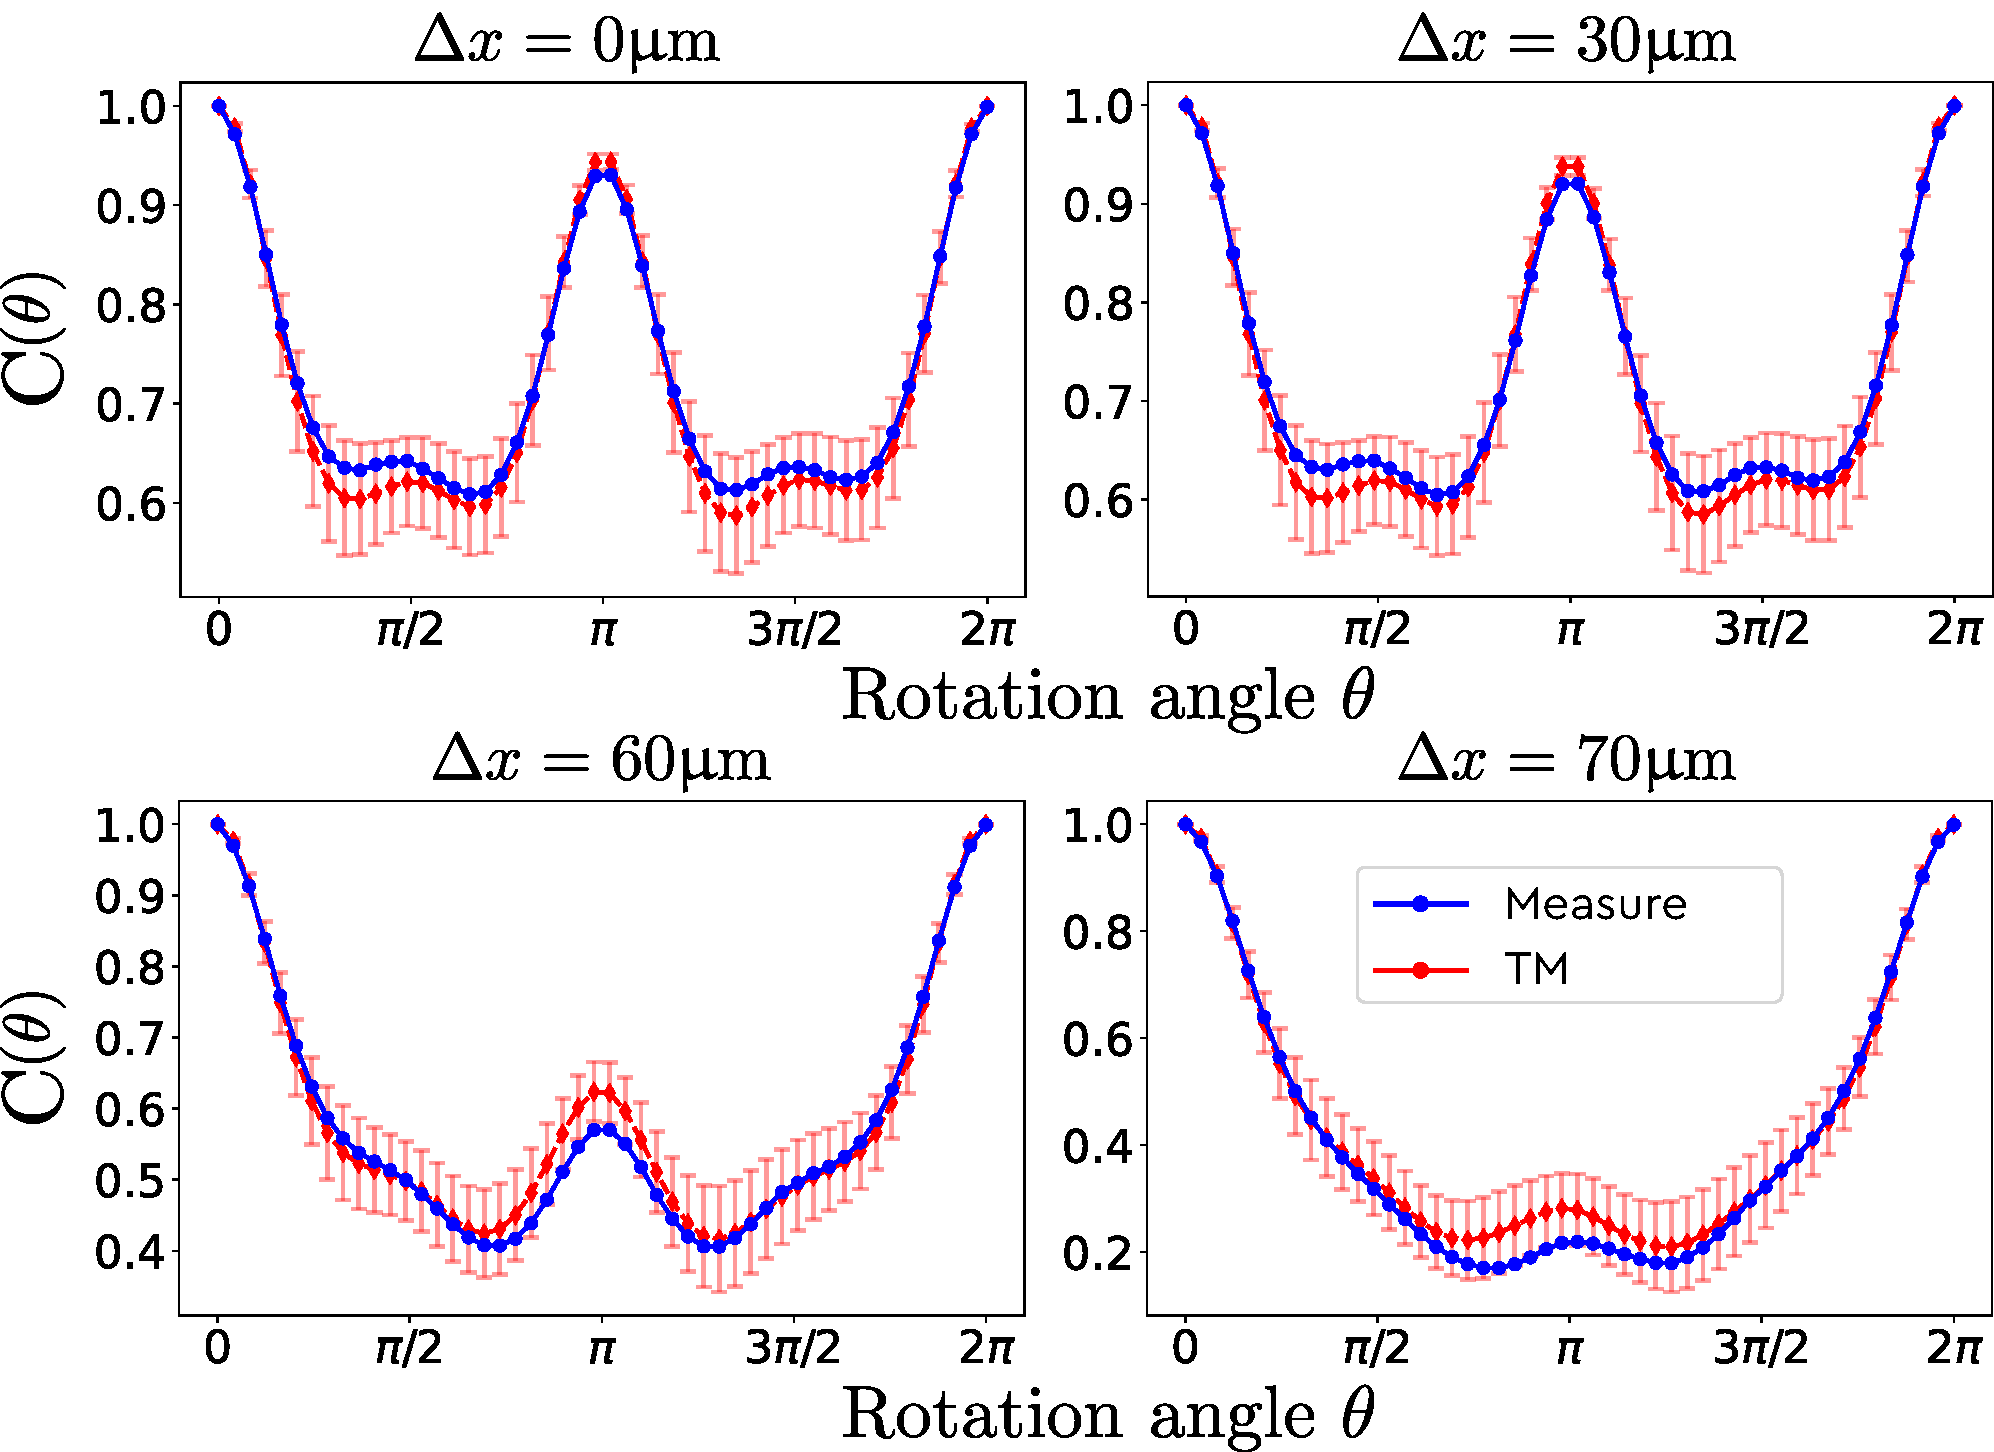
\includegraphics[width=0.49\textwidth]{images/Fig_A2.pdf}
\caption{
    \textbf{Comparison between the correlation measured and the one estimated using the TM.}
    For different values of the deformation, 
    we show the field correlation as defined in Eq.~\ref{eq:corr_function} (red curve), 
    and the one obtained using the TM (red curve).
}
\label{fig:TMvsCE}
\end{figure}

% \subsection*{Correlation for different output polarizations}

% \begin{figure}[ht]
% 
\includegraphics[width=0.35\textwidth]{images/placeholder.pdf}
% \caption{
%     \textbf{Correlation measurements for the cross-polarization configuration and for the total intensity (both polarizations).}
% }
% \label{fig:}
% \end{figure}


%%%%%%%%%%%%%%%%%%%%%%%%%%%%%%%%%%%%%%%%%%%%%%%%%%%%%%%%%%%%%%%%%%%%
%%%%%%%%%%%%%%%%%%%%%%%%%%% ANNEXE C %%%%%%%%%%%%%%%%%%%%%%%%%%%%%%%
%%%%%%%%%%%%%%%%%%%%%%%%%%%%%%%%%%%%%%%%%%%%%%%%%%%%%%%%%%%%%%%%%%%%
\section*{Appendix C: Model of disordered fibers}

In the following, we will make the approximations that:
1) we are in the weak coupling regime, 
allowing us to neglect the transverse component of the polarization and use the scalar wave equation,
2) we can disregard backreflections due to the effect of disorder,
and 
3) we can neglect coupling effects between propagating modes and non-propagating modes; 
this assumption will be respected far from the cut-off, i.e., not for the highest-order modes.
We consider one circular polarization of the field. 
The transverse part of the field, for an unperturbed axisymmetric index profile $n_0(\vec{r})$, 
satisfies the scalar Helmholtz equation:
% In the following, we will make the approximations that:
% 1) we are in the weak coupling approximation, allowing us to neglect the transversal component of the polarization and use the scalar wave equation,
% 2) we can neglect backreflections due to the effect of disorder,
% and 3) we neglect coupling effects between propagating modes and non-propagating modes, 
% this assumption will be respected far from the cut-off, 
% i.e. not for the highest-order modes.

% We consider one circular polarization of the field.
% The transverse part of the field, for an unperturbed axisymmetric index profile $n_0^2(\vec{r})$ satisfies the scalar Helmholtz equation:

\begin{equation}
    \left[ \frac{\partial^2}{\partial z^2} + \Delta_\perp + n_0(\vec{r})^2 k_0^2\right] \ket{\phi(\vec{r}, z)} = 0 \, .
    \label{eq:Helmholtz}
\end{equation}

% Considering only the propagation in the forward $z$ direction, we obtain~:

% \begin{equation}
%     \left[ \frac{\partial}{\partial z} + \nabla_\perp \cdot + n_0(\vec{r}) k_0\right] \ket{\phi(\vec{r}, z)} = 0 \, ,
%     \label{eq:Helmholtz_forward}
% \end{equation}

% with $\nabla_\perp \cdot = \frac{\partial}{\partial x} + \frac{\partial}{\partial y}$ the transverse part of the divergence operator.
% We are looking for the guided modes $\psi_\mu$ of the form~\cite{marcuse1982light}:

% \begin{equation}
%     \psi_\mu(\vec{r},z) =  \psi_\mu(\vec{r}) e^{i \beta_\mu z} =  a_\mu(r) e^{i m_\mu \theta} e^{i \beta_\mu z} \, ,
% \end{equation}



% with $\mu \in [0..N]$ and $N$ the total number of propagating modes.
% Injecting into Eq.~\ref{eq:Helmholtz_forward}, we have the relation

% \begin{equation}
%     \left[ \Delta_\perp + \left(n_0(\vec{r})^2 k_0^2 -\beta_\mu\right)\right] \ket{\psi_\mu} = 0 \, .
%     \label{eq:ideal_modes_Helm}
% \end{equation}

% In the weakly guided approximation, we have the orthogonality relation:

% \begin{equation}
%     \braket{\psi_\nu}{\psi_\mu} = \delta_{\mu,\nu}
%     \label{eq:mode_ortho}
% \end{equation}

% For a perturbed index profile $n(\vec{r}) = n_0(\vec{r}) + \delta n(\vec{r})$, 
% the wave equation becomes:

% \begin{equation}
%     \left[ \frac{\partial}{\partial z} + \nabla_\perp \cdot + n(\vec{r}) k_0\right] \ket{\phi} = 0 \, .
%     \label{eq:Helmholtz_forward_perturbed}
% \end{equation}

% Neglecting coupling to the non-propagating modes, 
% the solution for the field $\ket{\phi(\vec{r}, z)}$ can be expressed as a linear combination of the modes 
% $\ket{\psi_\mu(\vec{r}, z)}$ of the perfect fiber:

% \begin{equation}
%     \phi(\vec{r}, z) = \sum_\mu^N \alpha_\mu(z) \psi_\mu(\vec{r}, z) \, .
%     \label{eq:mode_decomp}
% \end{equation}



% Injecting Eq.~\ref{eq:mode_decomp} into Eq.~\ref{eq:Helmholtz_forward_perturbed}:

% \begin{equation}
% \begin{aligned}
%     \sum_\mu^N \alpha_\mu(z)\left[ \frac{\partial}{\partial z} 
%     + \nabla_\perp \cdot + n_0(\vec{r}) k_0\right] \ket{\psi_\mu}  \\
%     + \sum_\mu^N  \frac{\partial \alpha_\mu(z)}{\partial z} \ket{\psi_\mu} 
%     + \sum_\mu^N \alpha_\mu(z) \delta n(\vec{r}) k_0 \ket{\psi_\mu} =0 \, .
%     % \label{eq:Helmholtz_forward_perturbed}
% \end{aligned}
% \end{equation}

% The first term vanishes using Eq.~\ref{eq:ideal_modes_Helm}. 
% We now multiply on the left part by $\bra{\psi_\nu}$ and use the orthogonality relation (Eq~\ref{eq:mode_ortho}):

% \begin{equation}
%     \frac{\partial \alpha_\mu(z)}{\partial z}  
%     + \sum_\mu^N \alpha_\mu(z) k_0 \bra{\psi_\nu} \delta n(\vec{r})  \ket{\psi_\mu} =0 \, .
%     \label{eq:}
% \end{equation}

% We can rewrite this differential equation:

% \begin{equation}
%     \frac{\partial \boldsymbol{\alpha}(z)}{\partial z}  
%     + i k_0\mathbf{\Gamma}(z)\boldsymbol{\alpha}(z) =0 \, ,
%     \label{eq:}
% \end{equation}

% with $\boldsymbol{\alpha}(z)$ the vector of size $N$ containing the coefficients $\alpha_\mu(z)$, 
% and $\mathbf{\Gamma}(z)$ a matrix of size $N \times N$ containing the coupling coefficients

% \begin{equation}
% \mathbf{\Gamma}_{\nu \mu}(z) = \iint{}d\vec{r}  \delta n(\vec{r}, z) \psi_\nu^*(\vec{r})\psi_\mu(\vec{r})  e^{i \left( \beta_\mu-\beta_\nu\right)z} \, .
% \label{eq:gamma1}
% \end{equation}

% The solution is given by:

% \begin{equation}
%     \boldsymbol{\alpha}(z) = e^{ik_0\int_0^z dz' \mathbf{\Gamma}(z)} \boldsymbol{\alpha}(0)
% \end{equation}

% \subsection{Model of disorder}

% Let's now consider a disorder of the form

% \begin{equation}
% \delta n(\vec{r}, z) = f(z)g(r)h(\phi) \, .
% \end{equation}

%  We assume that the radial component of the disorder come from the fabrication process that consists in 
%  the deposition of layers of silica with varying concentration on dopant atoms. 
%  We can then consider that the index at a given radius $r$ can randomly vary between the index of the two neighbouring layers. 
%  For a given radius $r$, $g$ has a variance of the form:

%  \begin{equation}
%      \sigma_g(r) = d.\frac{dn_0(r)}{d r} \, ,
%  \end{equation}

%  \noindent with $d$ the layer thickness of the deposition, typically of the order of $1$nm (????).

%  For a graded-index fiber with a parabolic index profile, inside the core, we have:

%  \begin{equation}
%      \sigma_g(r) \propto  d \times \frac{r}{r_0^2}\, ,
%      \label{eq:var_g}
%  \end{equation}

% \noindent with $r_0$ the radius of the fiber.

%  Without loss of generality, we can consider the series expansion of the azimuthal function, 
%  and treat the case for 

 
%  \begin{equation}
%      h(\theta) = \gamma_q e^{i q \theta} \, ,
%  \end{equation}

%  with $q$ an integer value representing the orbital angular momentum of the deformation 
%  and $\gamma_q$ the corresponding weight.

%  Finally, we take $f(z)$ as a random function with a correlation width $l_z$. 
%  We can then approximate it as constant on segments of length $l_z$:

%  \begin{equation}
%      f(z) = f_p \quad \text{for} \quad z \in \left[ p\,l_z, (p+1)l_z \right]
%  \end{equation}

%  \subsection{Transmission matrix of a segment of length $l_z$}

% The transmission matrix linking the field in the section at $z = p\,l_z$ 
% to the one at $z = (p+1)l_z$ reads:
 
%  \begin{equation}
%      t_{\nu\mu}^p = e^{-i \beta_\mu l_z} \alpha_{\nu\mu}^p = e^{-i \beta_\mu l_z} \alpha_{\nu\mu}(z=pl_z) \, .
%  \end{equation}

%  with 

%  \begin{equation}
%      \alpha_{\nu\mu}^p = e^{-i k_0 \Gamma_{\nu\mu}^p} \, ,
%  \end{equation}

%  and

%   \begin{equation}
%      \Gamma_{\nu\mu}^p = 
%      \bra{\psi^\perp_\nu}\delta n_p(\vec{r})\ket{\psi^\perp_\mu)}
%      .e^{i\delta\beta_{\nu\mu}l_z} 
%      .\frac{\sin\left(\delta\beta_{\nu\mu}l_z/2\right)}{2\delta\beta_{\nu\mu}} \, ,
%  \end{equation}

%  with $\bra{\psi^\perp_\nu}$ the transverse part (in a plane orthogonal to the fiber axis) of the field of mode $\mu$.

%  \begin{equation}
%     \begin{aligned}
%      \bra{\psi^\perp_\nu}\delta n_p(\vec{r})\ket{\psi^\perp_\mu} &=&
%             \int r dr f_p(r) \psi^*_\nu(r) \psi_\mu(r)\\
%             &&\times \int d\theta e^{i\left(m_\nu-m_\mu+q\right)}\\
%             &=& \int r dr f_p(r) \psi^*_\nu(r) \psi_\mu(r)\\
%             &&\times \delta_{m_\nu-m_\mu+q}
%             \, .
%      \end{aligned}
%  \end{equation}

%  Then

%   \begin{equation}
%      t_{\nu\mu}^p = e^{i \beta_\mu l_z} \alpha_{\nu\mu}^p = e^{-i \beta_\mu l_z} \alpha_{\nu\mu}(z=pl_z) \, .
%  \end{equation}

%  Considering small deformations and small longitudinal correlation $l_z$ of the disorder, we have:

%   \begin{equation}
%      \alpha_{\nu\mu}^p \approx  \delta_{\mu\nu}  -i k_0 \Gamma_{\nu\mu}^p \, .
%  \end{equation}

% \subsection{TM of the full fiber}

%  Neglecting backreflections, we can multiply the TMs of each segment to obtain

%  \begin{equation}
%      t_{\nu\mu} \approx e^{-i \beta_\mu L} \left(
%         \mathbb {1}  -i k_0  \sum_p^N \Gamma_{\nu\mu}^p
%     \right)
%         \, .
%  \end{equation}

%  In particular, for the off-diagonal elements, 
%  \begin{equation}
%     \begin{aligned}
%      t_{\nu\neq\mu} &\propto& 
%              -e^{-i \beta_\nu L} k_0 l_z
%              .\delta_{m_\nu-m_\mu+q}
%              .\text{sinc}\left(\delta\beta_{\nu\mu}l_z/2\right)\\
%              &&\times \sum_p^N \int r dr f_p(r) \psi^*_\nu(r) \psi_\mu(r)
%         \, .
%         \end{aligned}
%  \end{equation}

% Variance of the elements of $t_{\mu\nu}$, using $N \approx L/l_z$:


%   \begin{equation}
%     \sigma^t_{\mu\neq\nu} \propto 
%         k_0L \, 
%         \delta_{m_\nu-m_\mu+q}
%         \left\lvert\text{sinc}\left(\delta\beta_{\nu\mu}l_z/2\right) \right\rvert
%         \bra{\psi^r_\nu}r\ket{\psi^r_\mu}
%         \, ,
%  \end{equation}

%  with $ \bra{\psi^r_\nu}r\ket{\psi^r_\mu} = \int r^2 dr \psi^*_\nu(r) \psi_\mu(r)$.\\

%  Observations:
%  \begin{itemize}
%     \item for a deformation $\delta n \propto sin\left(q\theta\right)$, we only 
%     have coupling between modes with an angular momentum difference $\pm q$,
%     \item for small deformations, the second term leads to significant coupling only for degenerate or quasi-degenerate modes.
%     \item the last term shows that the coupling term is more important the further away we are to the axis, 
%     which suggest that coupling will be more important for higher order modes where there is more energy away from the center of the core.
%  \end{itemize}


\subsection{Theoretical prediction of RME  correlation for weak disorder}

In the limit of weak disorder \new{DEMONSTRATION HERE},
we obtain



% \begin{equation}
%  A = (k_0 l_z)^2 \frac{L}{l_z} \frac{4}{3} \frac{(\Delta n)^2}{a N_\text{modes}}  d_\text{layer}^2
% \end{equation}

%%%%%%%%%%%%%%%%%%%%%%%%%%%%%%%%%%%%%%%%%%%%%%%%%%%%%%%%%%%%%%%%%%%%
%%%%%%%%%%%%%%%%%%%%%%%%%%% ANNEXE D %%%%%%%%%%%%%%%%%%%%%%%%%%%%%%%
%%%%%%%%%%%%%%%%%%%%%%%%%%%%%%%%%%%%%%%%%%%%%%%%%%%%%%%%%%%%%%%%%%%%
\section*{Appendix D: Effect of coupling in quasi-degenerate group of modes}

Small symmetric deformations ($q=0$) in graded-index fibers
lead, at the first order, to a global phase shift and subsequently
result in changes in the relative phase between the modes~\cite{BoonzajerFlaes2018robustness}. 
The TM matrix remains diagonal in the mode basis, 
thus it commutes with the rotation operator $\mathbf{R}(\theta)$ 
for all angles $\theta$.
As a result, it doesn't impact the RME.

When the amplitude of the deformation is strong, 
it populates the off-diagonal element of $\mathbf{T}$~\cite{matthes2021learning}.
This disrupts the ability of the rotation operator to commute with the TM~\cite{Li2021memory}.

In the regime between these two extreme cases, 
the system is governed by Eq.~\ref{eq:theo}. 
When the correlation length of the disorder in the $z$-axis, denoted as $l_z$,
is significantly larger than the wavelength, 
the coupling term's dependence on the difference $\delta\beta$ 
of the propagation constant in Eq.~\ref{eq:coupling} can be approximated, 
at the first order, 
by a Dirac function. 
This results in coupling only between pairs of quasi-degenerate modes.
% and thus results in the global decrease of the correlation function $C(\theta)$ observed.\\
% It can be explained by the fact that the dominant term due to the core-cladding distortion 
% couples preferentially modes with a difference of orbital angular momentum $\delta m = 2$ 
% and with a difference of propagation constant $\delta \beta \sim 0$. 
% It corresponds to coupling inside quasi-degenerate groups of modes. 
% If we assume only coupling between modes inside these groups, 
In this scenario, the TM matrix becomes block diagonal, 
enabling the problem to be addressed independently for each group of modes. 
For the $j^\text{th}$ group, we analyze the commutator between the relevant subpart of TM 
denoted as $\mathbf{T}_j$ for that group, 
and the rotation matrix $\mathbf{R}_j(\theta)$. 
Since, within each group, the angular momenta $m$ share the same parity 
(corresponding to $|m|+2l = cst$), 
it follows that $\mathbf{R}_j(\pi) = \pm \mathbb{1}$, 
where $\mathbb{1}$ represents the identity matrix, which commutes with all operators.

As a result, $\mathbf{R}_j(\theta = \pi)\mathbf{T}_j-\mathbf{T}_j\mathbf{R}_j(\theta= \pi) = 0$, 
regardless of the complexity of coupling within each group of modes. 
This provides an explanation for the observed robustness of the correlation peak at $\theta=\pi$.


%%%%%%%%%%%%%%%%%%%%%%%%%%%%%%%%%%%%%%%%%%%%%%%%%%%%%%%%%%%%%%%%%%%%
%%%%%%%%%%%%%%%%%%%%%%%%%%% ANNEXE E %%%%%%%%%%%%%%%%%%%%%%%%%%%%%%%
%%%%%%%%%%%%%%%%%%%%%%%%%%%%%%%%%%%%%%%%%%%%%%%%%%%%%%%%%%%%%%%%%%%%
\section*{Appendix E: Numerical simulations}

\subsection*{Principle}

To simulate the effect of small perturbation $\delta n$ of the refractive index, 
we perform simulations in Python, available in the dedicated repository~\cite{repo}. 
The steps are the following:
\begin{enumerate}
    \item We compute the mode profiles and propagation constant of the unperturbed fiber using the pyMMF package~\cite{matthes2021learning,pyMMF},
    \item we divide our fiber into segments of length $l_z$,
    \item for each segment indexed by $p$, we generate a radial and azimuthal disorder $\delta n_p(r,\phi)$ 
    following the model presented in the main text,
    \item we compute the matrix $\mathbf{V}$ representing the coupling introduced by that perturbation, 
    \item we add this perturbation to the unperturbed Hamiltonian $\mathbf{H}_0$ to find the TM of each segment, 
    \item finally, we multiply the TMs of all the segments to estimate the TM of the whole fiber.
\end{enumerate}

% We start by decomposing our fiber of total length $L=24.5$mm into segments of length $l_z$ 
% in which we consider the perturbation constant as a function of $z$ (see Eq.~\ref{eq:lz}). 
% We then estimate the transmission matrix of each slab for a disorder following the model. 
% The total TM of the system is obtained by multiplying the TMs of all the segments. 
% We finally compute the RME correlation coefficient defined in Eq.~\ref{eq:corr_function} 
% as a function of $\theta$
% by sending numerically $100$ random input wavefront and computing the output field.



\subsection*{Methods}



For each segment of length $l_z$ indexed by the integer $p$, 
we generate the matrix $\mathbf{V}^p$ representing the perturbation operator 
by projecting it into the previously computed modes of unperturbed fiber:

\begin{equation}
V^p_{\nu \mu} = \frac{2\pi}{\lambda} \bra{\psi_\nu} \delta n_p(r_j,\phi_i) \ket{\psi_\mu} = \bra{\psi_\nu} \delta n_p(r_j)  \delta n_p(\theta_i) \ket{\psi_\mu}
\end{equation}

% With $\delta n_p$ and $\mathbf{V}^p_\theta$ the radial and azimuthal components of the perturbation.



% \begin{equation}
% \mathbf{V}^p_{ji} = \mathbf{V}^p(\vec{r_j}, \vec{r_i}) = \mathbf{V}^p_r(\vec{r_j}, \vec{r_i})   \mathbf{V}^p_\theta (\vec{r_j}, \vec{r_i}) \, ,
% \end{equation}

The azimuthal term reads:

\begin{equation}
     \delta n_p(\theta) =  \sum_q \Gamma_q\cos(q \theta_i+\phi_{qi}) \, , 
\end{equation}

% \begin{equation}
%     \begin{aligned}
%         \mathbf{V}^p_{\theta_{ii}} &= \sum_q \Gamma_q\cos(q \theta_i+\phi_{qi}) \\
%         \mathbf{V}^p_{\theta_{i\neq j}} &= 0  
%     \end{aligned}
%     \, , 
% \end{equation}

with $\phi_{qi}$ is a random phase with a uniform distribution 
added to mitigate the effect of the orientation of the perturbation.\\

The radial term reads:

\begin{equation}
     \delta n_p(r_j) = \sigma(r_j) u_p(r_j) \, , 
\end{equation}

with $\sigma(r_j)$ as defined in the main and $u_p(r_j)$ 
a random Gaussian variable of mean $0$ and standard deviation $1$ 
on each ring of thickness $d_\text{layer}$.


% $
% \delta n_p(r,\phi) = g_p(r)\sum_q \Gamma_q\cos(q\phi)\ \text{for}\ z \in \left[ p\,l_z, (p+1)l_z \right].
% $


% We first generate a real diagonal random matrix $\mathbf{V}^p_r$
% with Gaussian statistics and variance 
% with a radial dependence given by Eq.~\ref{eq:var_g} 
% on a $N_{xy} = N_x.N_y$ Cartesian grid with $N_x = N_y = 64$. 
% It represents the radial dependence of the disorder in one segment.
% The azimuthal dependence of the disorder $\mathbf{V}_\theta$ 
% is also represented by a $N_{xy}\times N_{xy}$ diagonal matrix 
% with terms
% \begin{equation}
%    V^p_{\theta_{ii}} = \sum_q \gamma_q\cos(q \theta_i+\phi_q) \, ,
% \end{equation}

% \noindent with $i$ the index of an element of the Cartesian grid, 
% $\theta_i$ its azimuthal coordinate,
% and $\phi_i$ a random phase with a uniform distribution on $[0,2\pi]$.

% The total perturbation term then reads:
% \begin{equation}
%    \mathbf{V}(\vec{r})= \mathbf{V}^p_r\,  \mathbf{V}^p_\theta
% \end{equation}

% We then compute the spatial profiles and propagation constants 
% of the modes of a perfect graded-index fiber of radius 50\textmu m and numerical aperture $0.2$ 
% using the Python module PyMMF~\cite{pyMMF, matthes2021learning}. 
% It supports $N = 55$ modes per polarization. 
% In the scalar approximation, 
% considering only the TM between the input and output fields with the same circular polarization, 
% the TMs are of size $N\times N$. 
% The change of basis matrix $\mathbf{M}_0$ from the Cartesian grid to the mode basis  
% is a $N\times N_{xy}$ complex matrix.

% The transverse part $\bra{\psi^\perp_\nu}\delta n_p(\vec{r})\ket{\psi^\perp_\mu)}$ 
% of the coupling matrix $\mathbf{\Gamma}^p$ (Eq.~\ref{eq:gamma1}), 
% for a pair of input and output modes $\mu$ and $\nu$,
% is computed by projecting the perturbation  matrix $\mathbf{V}^p$ in the mode basis:

% \begin{equation}
%    \mathbf{\Gamma}_\perp^p = \mathbf{M}_0 \, \mathbf{V} \, \mathbf{M}_0^\dagger \, 
% \end{equation}

% with ${}^\dagger$ the Hermitian conjugate.

% The coupling contribution in Eq.~\ref{eq:gamma1} 
% accounting for the longitudinal dependence of the disorder
% is represented by the diagonal matrix $\mathbf{\Gamma}_z^p$ 
% with coefficients given by


% \begin{equation}
%    \mathbf{\Gamma}_{z_{\nu\mu}}^p = \frac{\sin\left(|\beta_{\mu}-\beta_\nu|l_z/2\right)}{2\delta|\beta_{\mu}-\beta_\nu|} \, .
% \end{equation}

The TM of segment $p$ is then computed using

\begin{equation}
   % \mathbf{T}^p =\mathbf{T}^p_0 e^{i \frac{2\pi}{\lambda}\mathbf{\Gamma}^p}  \, 
   \mathbf{T}^p = e^{\left(\mathbf{H}_0 + \mathbf{V}^p \right) l_z} \, ,
\end{equation}

$\mathbf{H}_0$ is a diagonal matrix containing the propagation constant of each mode, 
it represents the Hamiltonian of the perfect fiber.\\

% \noindent with $\mathbf{T}^p$ a diagonal matrix with $\mathbf{T}^p_{0_{\mu\mu}} = e^{i \beta_\mu \left(l_z+l^p_\text{rnd}\right)}$.
% The  small random length $l^p_\text{rnd}$ with uniform distribution on $[0,2\lambda]$
% is added to avoid spurious coherent effects that could appear with segments of constant size $l_z$.

Finally, the TM of the full fiber is obtained using

\begin{equation}
   \mathbf{T}^p = \prod_p^{N_z}  \mathbf{T}^p  \, .
\end{equation}

% \begin{equation}
%     \mathbf{O}(\theta_t) = \mathbf{T}^\dagger\mathbf{R(\theta_t)}^\dagger\mathbf{T}\mathbf{R(\theta_t)}.
% \end{equation}

%%%%%%%%%%%%%%%%%%%%%%%%%%%%%%%%%%%%%%%%%%%%%%%%%%%%%%%%%%%%%%%%%%%%
%%%%%%%%%%%%%%%%%%%%%%%%%%% ANNEXE F %%%%%%%%%%%%%%%%%%%%%%%%%%%%%%%
%%%%%%%%%%%%%%%%%%%%%%%%%%%%%%%%%%%%%%%%%%%%%%%%%%%%%%%%%%%%%%%%%%%%
\section*{Appendix F: RME Characterization of different GRIN fibers}

We additionally reproduce the measurement for other
fiber segments of the same length (24.5cm)
and with similar advertised properties.
We use samples from a 
Thorlabs 50-micron core OM2 graded-index fiber (GIF50C, NA = 0.2).

Results were reproducible for different fiber segments of the same spool. 
We present typical results for one sample in Fig.\ref{fig:tl1}.
We observe different contributions of the $cos(q\theta)$ terms 
compared to Fig.~\ref{fig:theoryVSexpVSsimu} with the BendBright OM4 fiber.
In particular, $\Gamma_4$ is much lower,
leading to the absence of observed local maxima
of the correlation at $\pi/2$ and $3\pi/2$.


\begin{figure}[ht]
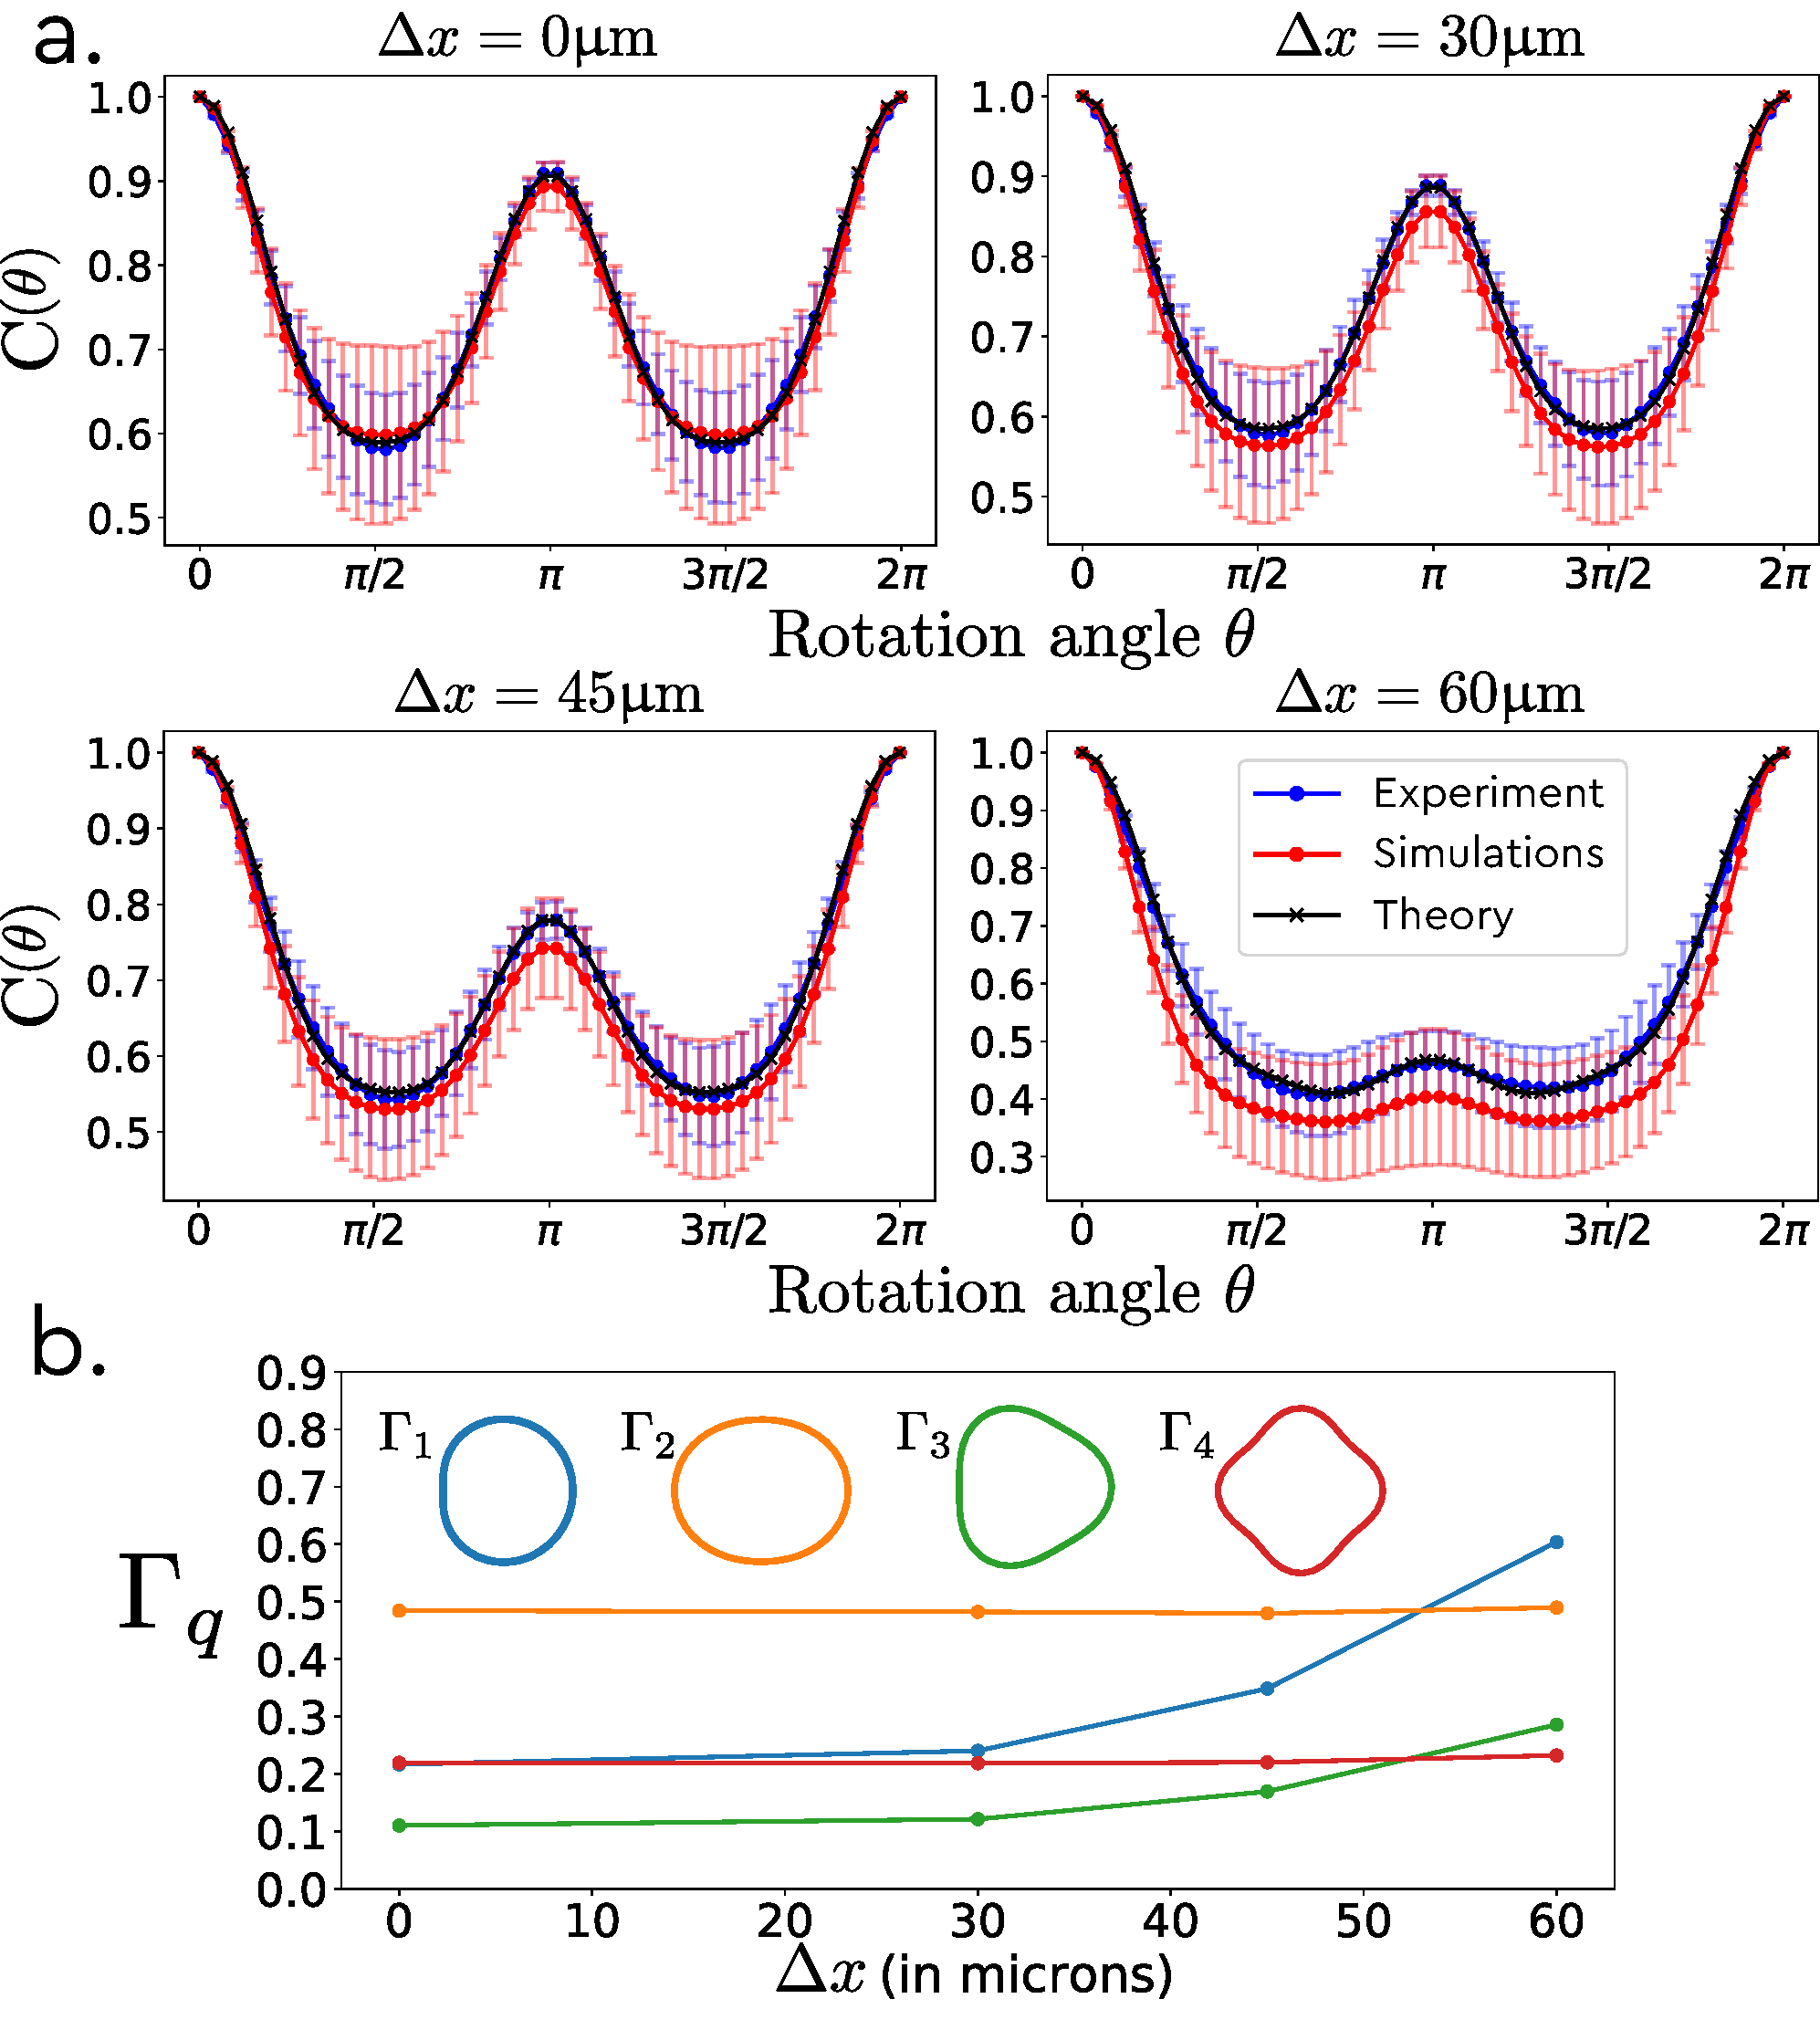
\includegraphics[width=0.49\textwidth]{images_si/Fig_GRIN3.pdf}
\caption{
\textbf{RME correlation results for GIF50C batch 1.}
    a, Correlation curves of the RME, as defined in Eq.~\ref{eq:corr_function},
    for various levels of deformation:
    experimental data (blue),
    fit of the model using Eq.~\ref{eq:theo} (black),
    and simulation results using the same parameters as those for the theoretical model fit (red).
    b, Values of the deformation parameters $\Gamma_q$ found by fitting
    the theoretical model to the experimental data
    as a function of the deformation.
    In the insert, we show the symmetry corresponding to the perturbation associated with each value of $q$.
}
\label{fig:tl1}
\end{figure}

%%%%%%%%%%%%%%%%%%%%%%%%%%%%%%%%%%%%%%%%%%%%%%%%%%%%%%%%%%%%%%%%%%%%
%%%%%%%%%%%%%%%%%%%%%%%%%%% ANNEXE G %%%%%%%%%%%%%%%%%%%%%%%%%%%%%%%
%%%%%%%%%%%%%%%%%%%%%%%%%%%%%%%%%%%%%%%%%%%%%%%%%%%%%%%%%%%%%%%%%%%%
\section*{Appendix G: Autocorrelation of the RME channels}


As articulated in the primary text, for the effective retrieval of information from the far side of a complex medium, 
the utilized output pattern should possess both a substantial memory effect range and a narrow autocorrelation function. 
In the context of the Random Medium Effect (RME), this implies that 
$C(\theta)$ from Equation~\ref{eq:corr_function} displays a broad width, 
and the angular autocorrelation $C_0(\theta)$ is sharply peaked, with

\begin{equation}
    C_0(\theta) =  
        \left|
        \frac{
            \bra{\phi}\mathbf{T}^\dagger\mathbf{R(\theta)}^\dagger\mathbf{T}\ket{\phi}
        }{
                \bra{\phi}\mathbf{T}^\dagger\mathbf{T}\ket{\phi}        
        }
        \right|
    \, .
\end{equation}

We present in Fig.\ref{fig:autocorr} the autocorrelation of the first two RME channels, 
employing both the operators $\mathbf{O}(\theta_t= \pi/2)$ and the sum operator $\mathbf{O}_\text{sum}$ 
(as per Eq.\ref{eq:RME_sum_op}), 
as well as the first two fiber modes under varying conditions 
— absence of external deformations and presence of strong deformations. 
As anticipated, the fundamental mode, being less susceptible to perturbations, 
exhibits a rotational symmetry with a strong correlation across the entire angular range, 
even under significant deformations. 
The first open channels, 
which display a pattern resembling the fundamental mode 
(refer to insets in Fig.~\ref{fig:tailoring}), 
embody this property to a reduced extent.
This indicates that, despite their potent RME and expansive angular range, 
they do not fulfill the criteria to be viable candidates for image or information retrieval. 
However, the second channels do exhibit a pronounced RME peak around $\theta = 0$. 
In the case of $\mathbf{O}_\text{sum}$, the autocorrelation becomes flat with a correlation value close to 0. 
In conjunction with the extensive RME angular range, 
they present the potential to be utilized effectively to discern angular properties of an object 
or signal obscured at the fiber's distal end, 
leveraging the approach developed in scattering media~\cite{bertolotti2012non-invasive}.



\begin{figure}[ht]
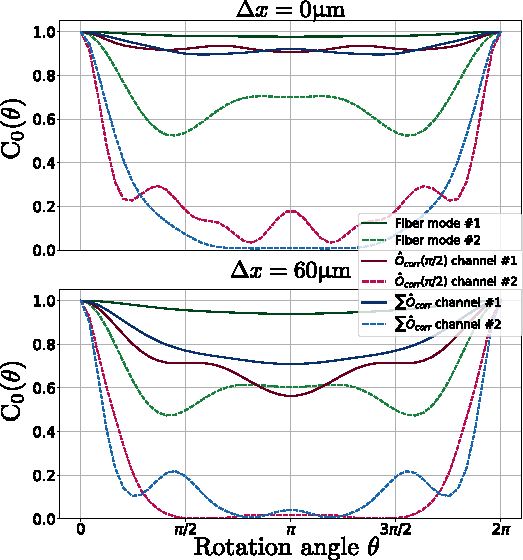
\includegraphics[width=0.49\textwidth]{images/Fig_F_C0.pdf}
\caption{
\textbf{Autocorrelation of the RME channels.}
Blabla
}
\label{fig:autocorr}
\end{figure}

% \section*{Appendix: The commutation operator to maximize the RME for a given angle}

% As the RME reflects the ability of the TM to commute with the rotation operator $\mathbf{R}(\theta)$, 
% a first choice is to study the commutation operator

% \begin{equation}
%     \mathbf{R}(\theta)\mathbf{T}-\mathbf{T}\mathbf{R}(\theta)
% \end{equation}

% By performing a singular value decomposition and choosing the singular vector 
% associated with the lowest singular value, 
% we find the input channels $\ket{\phi^c}$
% that minimizes the error difference between the output speckles 
% when the rotation is applied before and after the propagation. 
% We show in Fig.\ref{fig:tailoring} the experimentally measured correlation $C(\theta)$
% when sending and rotation the optimal wavefront for angles $\theta = \pi/2$ and $\theta = 3\pi/2$ 
% for different values of the perturbation 
% (green and yellow curves). 
% We see that the correlation presents a second maximum at the optimized angle value, 
% but also shows an overall correlation above the average one. 

% \nocite{*}

\bibliography{biblio}% Produces the bibliography via BibTeX.

\end{document}
%
% ****** End of file apssamp.tex ******
